% Document layout
\documentclass[a4paper,11pt]{article}
\usepackage[a4paper, inner=2.5cm , outer=2.5cm, top=2cm, bottom=2cm]{geometry}
\usepackage[usenames,dvipsnames]{color}
% Referencing & fonts
\usepackage[sort&compress]{natbib}
\setlength{\bibsep}{0.0pt}
\usepackage[font=small,labelfont=bf]{caption}
\usepackage[OT2,T1]{fontenc}
% Set formats for each heading level
\usepackage{sectsty}
\allsectionsfont{\usefont{OT1}{phv}{bc}{n}\selectfont}
\sectionfont{\color{MidnightBlue}} % sets colour of sections
\subsectionfont{\color{MidnightBlue}}  % sets colour of subsections
\subsubsectionfont{\color{MidnightBlue}}  % sets colour of subsections
% Other shit
\usepackage{algorithm}
\usepackage{amsfonts}
\usepackage{amsmath}
\usepackage{amssymb}
\usepackage{bbm}
\usepackage{booktabs}
\usepackage{epsfig}
\usepackage{float}
\usepackage[font=normalsize]{caption}
\usepackage{graphicx}
\usepackage{hyperref}
\usepackage{lineno}
\usepackage{mathtools}
\usepackage{sidecap}
\usepackage{sectsty}
\usepackage{verbatim}
\usepackage{wrapfig}
\usepackage{xcolor}
% Declarations
\DeclarePairedDelimiter\floor{\lfloor}{\rfloor}
\DeclareSymbolFont{cyrletters}{OT2}{wncyr}{m}{n}
\DeclareMathSymbol{\Sha}{\mathalpha}{cyrletters}{"58}
\DeclareMathSymbol{\sha}{\mathalpha}{cyrletters}{"57}
% Defined commands
 \newcommand{\prgname}[1]{\textcolor{NavyBlue}{\texttt{#1}}}
 \newcommand{\linkfont}[1]{\textcolor{BurntOrange}{\textbf{#1}}}
\newcommand{\shellcmd}[1]{\\\indent\indent\texttt{\$ #1}}
\newcommand{\shellctd}[1]{\\\indent\indent\texttt{#1}}
\newcommand{\ra}[1]{\renewcommand{\arraystretch}{#1}}
\begin{document}
\begin{figure}
\centering
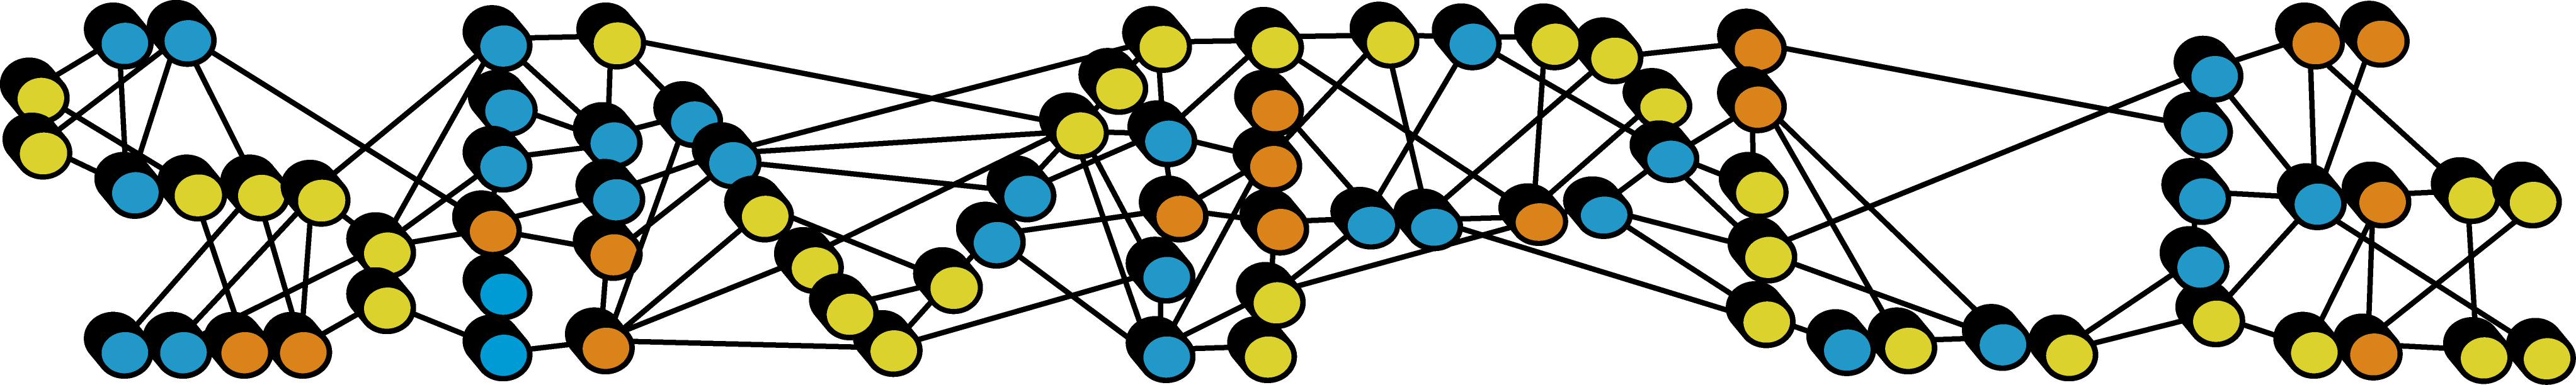
\includegraphics[keepaspectratio=true,scale=0.6]{./SIMPLE_logo/rawlogo}
%\caption{}
\end{figure}

\title{\prgname{The SIMPLE 3.0 Manual}}
\date{May 15, 2016}
\maketitle

\vspace{1em}
\begin{minipage}[ht]{0.48\textwidth}
www.simplecryoem.com\\
hans.elmlund@monash.edu\\
dominika.elmlund@monash.edu\\
Dept. Biochemistry and Molecular Biology\\
School of Biomedical Sciences\\
Monash University, Bldg. 77\\
Clayton, VIC, Australia, 3800\\
\end{minipage}
\vspace{20pt}

\begin{quote}
\textbf{"Keep it SIMPLE stupid"}\\(\textit{Kelly Johnson}; lead engineer at the Lockheed Skunk Works, coined the famous KISS principle stating that systems work best if they are kept simple rather than made complex. Therefore, simplicity should be a key goal in design and unnecessary complexity should be avoided.)
\end{quote}

\begin{quote}
\textbf{"Everything should be made as SIMPLE as possible, but no SIMPLEr"}\\(\textit{Albert Einstein})
\end{quote}

\begin{quote}
\textbf{"Complex theories do not work, SIMPLE algorithms do"}\\(\textit{Vladimir N. Vapnik}; author of \textit{The Nature of Statistical Learning Theory})
\end{quote}
\clearpage

\tableofcontents{}
\clearpage

\section{About SIMPLE}

\textbf{S}ingle-particle \textbf{IM}age \textbf{P}rocessing \textbf{L}inux \textbf{E}ngine (\href{www.simplecryoem.com}{\textbf{\textcolor{BurntOrange}{SIMPLE}}}) is a program package for cryo-EM image processing, focusing on \textit{ab initio} 3D reconstruction of low-symmetry single-particles. The SIMPLE back-end consists of an object-oriented numerical library written in modern Fortran. The SIMPLE front-end consists of a few standalone, interoperable components developed according to the "Unix toolkit philosophy".

SIMPLE is free software: you can redistribute it and/or modify it under the terms of the \href{http://www.gnu.org/copyleft/gpl.html}{\textbf{\textcolor{BurntOrange}{GNU General Public License}}} as published by the Free Software Foundation, either version 3 of the license, or (at your option) any later version. SIMPLE is distributed with the hope that it will be useful, but WITHOUT ANY WARRANTY; without even the implied warranty of MERCHANTABILITY or FITNESS FOR A PARTICULAR PURPOSE. See the \href{http://www.gnu.org/copyleft/gpl.html}{\textbf{\textcolor{BurntOrange}{GNU General Public License}}} for more details.

\subsection{What is new in SIMPLE release 2.1?}

Our \textbf{PRIME} (for \textbf{PR}obabilistic \textbf{I}nitial \textbf{M}odel generation for single-particle cryo-\textbf{E}lectron microscopy) code has undergone major revisions. First, we re-cast the original PRIME algorithm into an approach for solving  the problem of Simultaneous 2D Alignment and Clustering (SAC) \citep{reboul2016stochastic}. The PRIME SAC solver, implemented in the program \prgname{simple\_prime2D}
\begin{itemize}
    \item[--] generates improved 2D class averages from large single-particle cryo-EM datasets
    \item[--] can be used in conjunction with \prgname{simple\_prime3D} to obtain a reliable 3D starting model in a rapid and unbiased fashion
    \item[--] overcomes inherent limitations in widely used clustering approaches, such as initialisation bias and local optimality
    \item[--] is many times faster than other widely used approaches
\end{itemize}
Secondly, the program \prgname{simple\_prime3D} implements a revised version of our \textit{ab initio} 3D reconstruction code that is about 150 times faster than the previously released version. This speedup was accomplished using new theory for fast rotational matching of polar Fourier transforms based on Hadamard products calculated using a re-organised and highly parallelizable data structure. The paper describing this is not yet published, but we have release the code since we anticipate that the massive speedup will have major impacts for our users. For example, less than 10,0000 particles downscaled to about 100x100 pixels can feasibly be processed on a modern laptop equipped with an Intel i5 or i7 processor. We executed an \textit{ab initio} 3D reconstruction run using PRIME3D on half a million images downscaled to 64x64 pixels in less than 5 hours on a cluster with 224 CPU cores (Intel(R) Xeon(R) CPU E5-2670 0 @ 2.60GHz).

\section{File Formats}

SIMPLE2.1 supports both SPIDER (\texttt{*.spi}) and MRC (\texttt{*.mrc}) formats for image stacks and volumes. The MRC file handling classes are shared with the the Frealix program for helical reconstruction \citep{rohou2014frealix}. Relion \citep{Scheres:2012aa} uses the convention that MRC stacks have the suffix \texttt{*.mrcs} and volumes the suffix \texttt{*.mrc}. This is to overcome the annoyance that it is not possible to tell from an MRC file header whether a MRC file is a volume or a stack. With SIMPLE you can select to use either the \texttt{*.mrcs} or \texttt{*.mrc} suffix for stacks. The way that we keep track of whether a file is a volume or stack is via the command line key value. The key-value pairs \texttt{vol1=rec.mrc} and \texttt{vol2=rec2.mrc} refer to volumes whereas the key-value pairs \texttt{stk=ptcls.mrc} and \texttt{stk2=ptcls2.mrc} refer to stacks. Another notable change is the text file format used to write per-particle information to disk. The SIMPLE text-files used for parameter input/output now use a \texttt{key=value} syntax of the form
\begin{verbatim}
    e1=80. e2=100. e3=5.5 x=1.23 y=4.25 dfx=2.56 dfy=2.54 angast=30.5 state=1
\end{verbatim}
to represent per-particle information. Internally, the orientation information is stored in a dynamic hash data structure, which gives the file format high flexibility. Therefore, writing conversion scripts to allow interchange of parameters between SIMPLE and other packages is trivial. SIMPLE uses the same conventions as Frealign \citep{Grigorieff:2007aa} to represent orientations and CTF parameters. The CTF parameterization obtained by CTFFIND \citep{Mindell:2003aa} can be directly plugged into SIMPLE, for example by creating a file \texttt{deftab.txt}, looking like:
\begin{verbatim}
    dfx=2.56 dfy=2.76 angast=30.5
    dfx=3.50 dfy=3.33 angast=60.0
    dfx=1.98 dfy=2.02 angast=120.5
    ...
\end{verbatim}
and adding \texttt{deftab=deftab.txt} and \texttt{ctf=yes} to the PRIME command line (if the images are phase-flipped, this should be indicated by \texttt{ctf=flip}). The \texttt{SIMPLE/scripts} folder contains a perl-script (\texttt{convert\_frealign2simple.pl}) to convert a Frealing parameter file to a SIMPLE parameter file. This is easy, since both software internally use the \href{http://spider.wadsworth.org/spider_doc/spider/docs/euler.html}{\textbf{\textcolor{BurntOrange}{Spider Euler angle convention}}}. Other packages may use other conventions.

\section{Installation}
\label{install}

\subsection{System requirements}
\label{sysreq}

\subsubsection{Hardware}
\label{hardware}

\begin{itemize}
	\item [CPU]
	\begin{itemize}
		\item[--] Linux (fully supported Debian-based distributions: Mint-17.1, Ubuntu (14.10, 15.04, 15.10, 16.04 LTS)), SUSE-13.2 (earlier SUSE versions are also supported but not tested)
		\item[--] MacOSX (Yosemite and El Capitan, i.e. 10.10 and above)
	\end{itemize}
\end{itemize}

\subsubsection{Software}
\label{soft}

\begin{itemize}
	\item [CPU]
	\begin{itemize}
		\item[--] GNU tool chain 4.9 and above.
		\item[--] The linear algebra packages: Lapack and BLAS
		\item[--] FFTW-3 (The Fastest Fourier Transform in the West library)
	\end{itemize}
\end{itemize}


\subsection{Compiling from source on a Linux PC}
\label{compilepc}

Here we will compile SIMPLE2.1 from source on a Linux PC. The manual states that  SIMPLE2.1 requires the GNU toolchain version 4.9.1 or later (see above). Although SIMPLE supports all newer versions of the GNU toolchain, it is safest to use version 4.9.X because later versions are currently incompatible with the CUDA7 compiler. GPU accelerated code is planned for SIMPLE v3 and it may not be supported unless 4.9.X is used. To check the compiler versions, we execute
\begin{verbatim}
    $ gfortran --version
    GNU Fortran (GCC) 4.9.1
    Copyright (C) 2014 Free Software Foundation, Inc.
\end{verbatim}
To confirm that the gcc and g++ compilers are of the same version, we execute
\begin{verbatim}
    $ gcc --version
    gcc (GCC) 4.9.1
    Copyright (C) 2014 Free Software Foundation, Inc.
    This is free software; see the source for copying conditions.  There is NO
    warranty; not even for MERCHANTABILITY or FITNESS FOR A PARTICULAR PURPOSE.
\end{verbatim}
\begin{verbatim}
    $ g++ --version
    g++ (GCC) 4.9.1
    Copyright (C) 2014 Free Software Foundation, Inc.
    This is free software; see the source for copying conditions.  There is NO
    warranty; not even for MERCHANTABILITY or FITNESS FOR A PARTICULAR PURPOSE.
\end{verbatim}
To check whether lapack is installed, we open the package manager installed on our system (in our case \texttt{Synaptic} but other systems may have others, such as \texttt{YaST}, \texttt{apt} etc.) and search for \texttt{lapack} and see that \texttt{liblapack3} is installed on the system. We also search for \texttt{fftw} and see that the \texttt{libfftw3-single-3} is installed on the system. We cd to the directory  where we have our software installed (\texttt{<my software location>}) and copy the tar ball there
\begin{verbatim}
    $ cd <my software location>
    $ cp ~/Downloads/simple2.1.tar.gz .
\end{verbatim}
Next, we unpack the tar ball and cd to the simple directory
\begin{verbatim}
    $ gunzip simple2.1.tar.gz
    $ tar -xvf simple2.1.tar
    $ cd simple2.1/
\end{verbatim}
To check which Linux distribution we are running, we execute
\begin{verbatim}
    $ lsb_release -a
    No LSB modules are available.
    Distributor ID: Ubuntu
    Description:    Ubuntu 15.10
    Release:    15.10
    Codename:   wily
\end{verbatim}
Now we try to identify the configuration template file most suitable for our system by executing
\begin{verbatim}
    $ ls -1 scripts/Template_*
    scripts/Template_FEDORA_21x64_CPU_simple_user_input.pm
    scripts/Template_MacOSX_10.9.5x64_CPU_simple_user_input.pm
    scripts/Template_MacOSXFINK_10.11.4x64_CPU_simple_user_input.pm
    scripts/Template_MASSIVE_CPU_simple_user_input.pm
    scripts/Template_Mint_17.1x64_CPU_simple_user_input.pm
    scripts/Template_OXFORD_CPU_simple_user_input.pm
    scripts/Template_SUSE_13.2x64_CPU_simple_user_input.pm
    scripts/Template_Ubuntu_14.10x64_CPU_simple_user_input.pm
    scripts/Template_Ubuntu_15.10x64_CPU_simple_user_input.pm
    scripts/Template_Ubuntu_16.XXx64_CPU_simple_user_input.pm
\end{verbatim}

For this system, it looks like the \texttt{Template\_Ubuntu\_15.10x64\_CPU\_simple\_user\_input.pm} is the best fit, so we copy it to the root of the SIMPLE directory and rename it by executing
\begin{verbatim}
    $ cp ./scripts/Template_Ubuntu_15.10x64_CPU_simple_user_input.pm
    simple_user_input.pm
\end{verbatim}

We open the \texttt{simple\_user\_input.pm} file in our favourite text editor (vim) and replace on line 30 \texttt{our\$SIMPLE\_PATH$=$"/mysimplepath/"} with \texttt{our\$SIMPLE\_PATH$=$"<my software location>/simple2.1/"}. This is the path in which the software will be installed. We close vim and execute
\begin{verbatim}
    $ ./Makefile_genAll.pl
    SIMPLE library has finished compilation in dir:
    <my software location>/simple2.1
    *********************************************************
    * Compilation and linkage is complete for Simple-v2.1   *
    * You may run all simple checks  --- List check options *
    * > make check                   --- > make check_help  *
    *                                --- > make check_cpu   *
    * Cleaners: --- > make {clean,cleanall,clean_check_cpu} *
    * New Rel.: --- > make checknews                        *
    * Lne Cntr: --- > make wc                               *
    *********************************************************
\end{verbatim}

Compilation was succesful and we see that a new directory \texttt{/bin} has been created in the simple directory in addition to two text files \texttt{add2.bashrc} and \texttt{add2.tcshrc}
\begin{verbatim}
    $ cat add2.bashrc
    export SIMPLEPATH=<my software location>/simple2.1/
    export PATH=${SIMPLEPATH}/scripts:${SIMPLEPATH}/$PATH
    $ cat add2.tcshrc
    setenv SIMPLEPATH <my software location>/simple2.1/
    set path=(${SIMPLEPATH}/scripts ${SIMPLEPATH}/bin $path)
\end{verbatim}

On this machine we use the bash shell, so we add the lines in \texttt{add2.bashrc} to the \texttt{.bashrc} file and when a new terminal window is opened we have access to all the \texttt{simple\_*} programs.

\subsection{Compiling from source on MacOSX}
\label{compilemac}

This procedure is virtually identical to the one described for Linux above but we need to select the correct configuration file. If the \texttt{fink} package manager was used to install the GNU toolchain and the FFTW library, try the configuration file:
\begin{verbatim}
    scripts/Template_MacOSXFINK_10.11.4x64_CPU_simple_user_input.pm
\end{verbatim}
 Otherwise, try the file:
\begin{verbatim}
    scripts/Template_MacOSX_10.9.5x64_CPU_simple_user_input.pm
\end{verbatim}

\subsection{Compilation troubleshooting}
\label{compiletrouble}

\subsubsection{FFTW, Lapack and BLAS}

If not already installed, the FFTW-3 library needs to be installed. Most Linux package managers \texttt{YaST}, \texttt{Synaptic}, \texttt{apt-get} etc. provide the FFTW-3 library. On a Mac system the \texttt{Fink} and \texttt{Macports} package managers provide the FFTW-3 library or it can be obtained from: \url{http://www.fftw.org/install/mac.html}. SIMPLE relies on the single-precision FFTW library. Typically we will need to
\begin{verbatim}
    $ ./configure --enable-floats
    $ make
    $ sudo make install
\end{verbatim}

The \texttt{--enable floats} directive is critical as the installer will otherwise only install the double-precision version of the library. We check that we have in the lib folder (typically: \texttt{/usr/local/lib/}):

\begin{verbatim}
    libfftw3.a libfftw3.la
    libfftw3f.a libfftw3f.la
\end{verbatim}

Similarly the \texttt{lapack3} and \texttt{BLAS} will need to be installed on the system. On MacOSX Lapack and BLAS are usually installed by default. Installation of the dependencies on a PC with a Debian operating system, such as Ubuntu or Mint, is done using the \texttt{apt-get install} command as a super user
\begin{verbatim}
    #the compilers
    $ sudo apt-get install gfortran gfortran-4.9 gcc-4.9 g++-4.9
    #libraries (Lapack and BLAS)
    $ sudo apt-get install scalapack-doc scalapack-mpi-test
    scalapack-pvm-test scalapack-test-common  libscalapack-pvm1
    libscalapack-pvm-dev libscalapack-openmpi1 libopenblas-base
    libopenblas-dev libmlpack-dev libblas-dev libblas3 liblapack-dev
    liblapack-doc liblapack-doc-man liblapack3 libopenmpi-dev
    libmeep-mpich2-dev
    #FFTW-3
    $ sudo apt-get install libfftw3-bin libfftw3-dbg libfftw3-dev
    libfftw3-doc libfftw3-double3 libfftw3-long3 libfftw3-quad3
    libfftw3-single3 cl-fftw3 fftw-dev fftw-docs libfftw3-3
    libfftw3-mpi-dev libfftw3-mpi3 
\end{verbatim}

\subsubsection{Compilers}

One possible cause of failing compilation may be that the compiler paths are not correctly set in the \texttt{simple\_user\_input.pm} file. A typical compiler configuration on Ubuntu looks like
\begin{verbatim}
    our$CC_COMPILER = "gcc-4.9";
    our$GCC_COMPILER = "g++-4.9";
    our$MPI_F_COMPILER = "/usr/bin/mpif90";
    our$FCOMPILER = "gfortran-4.9";
\end{verbatim}
A configuration on MacOSX could look like
\begin{verbatim}
    our$CC_COMPILER = "/usr/local/bin/gcc";
    our$GCC_COMPILER = "/usr/local/bin/g++";
    our$MPI_F_COMPILER = "/usr/local/bin/mpif90";
    our$FCOMPILER = "/usr/local/bin/gfortran";
\end{verbatim}

If we used the \texttt{Fink} package manager to install the GNU toolchain on MacOSX, the configuration will typically look like:

\begin{verbatim}
    our$CC_COMPILER = "/sw/bin/gcc-fsf-5";
    our$GCC_COMPILER = "/sw/bin/g++-fsf-5";
    our$MPI_F_COMPILER = "/sw/bin/mpif90";
    our$FCOMPILER = "/sw/bin/gfortran";
\end{verbatim}

If we are on MacOSX and used the \texttt{MacPorts} package manager to install the GNU toolchain, the configuration will typically look like:

\begin{verbatim}
    our$CC_COMPILER = "/opt/local/bin/gcc";
    our$GCC_COMPILER = "/opt/local/bin/g++";
    our$MPI_F_COMPILER = "/opt/local/bin/mpif90";
    our$FCOMPILER = "/opt/local/bin/gfortran";
\end{verbatim}

On MacOSX it is required that the correct Command Line Tools for \texttt{Xcode} are installed. If we use the package managers \texttt{Fink} or \texttt{MacPorts} this is taken care of as part of the installation procedure. The \texttt{gfortran-5},  \texttt{gcc-5} and \texttt{g++-5} compilers can be installed via the \texttt{apt-get}, \texttt{Synaptic} or \texttt{YaST} package managers on Linux systems. Beware that Apple have their own gcc compiler (for objective-C) which is different than the GNU one and will generate errors upon compilation.

\begin{verbatim}
    $ gcc --version 
    Configured with: --prefix=/Applications/Xcode.app/Contents/Developer/usr
    --with-gxx-include-dir=/usr/include/c++/4.2.1
    Apple LLVM version 6.0 (clang-600.0.54) (based on LLVM 3.5svn)
    Target: x86_64-apple-darwin13.4.0
    Thread model: posix
\end{verbatim}

The compilation needs to be using the GNU compiler and \textbf{\textit{not}} the Apple one. Otherwise the compilation will not work. Make sure that the paths in \texttt{simple\_user\_input.pm} are pointing to the correct location

\begin{verbatim}
    $SIMPLE_PATH= {path where simple will be installed}
    $CC_COMPILER = {path to the gcc compiler on MacOSX,
                     default: /usr/local/bin/gcc}
    $GCC_COMPILER = {path to the g++ compiler on MacOSX,
                     default: /usr/local/bin/g++}
    $MPI_F_COMPILER = {path to the mpif90 compiler on MacOSX, 
                       default:/usr/local/bin/mpif90}
    $FCOMPILER = {path to the gfortran or ifort compiler on MacOSX,
                   default: /usr/local/bin/gfortran}

    $MPI_DIR={path to the mpi directory, default:/usr}
    $MPI_DIR_INCLUDE="/usr/include/mpi";
    $FFTW_LIB={path for to the FFTW lib, default: /usr/local/lib}
    $FFTW_INC={path to the include for the FFTW, default:
    /usr/local/fftw/3.3.4-gcc/include/} cluster dependent

    $OBJDIR={path to the object compiled files, default: obj/GFORTgpu}
    $MODDIR={path to the .mod files, default: obj/GFORTgpu}
\end{verbatim}
All of the compilers must originate from the same version of the GNU toolchain.

\subsection{Installation on a Linux cluster}
\label{inst_clusters_linux}

Installation on a Linux cluster is essentially the same as on a Linux workstation with the exception that the appropriate modules need to be loaded before installation and execution. On a typical SLURM cluster

\begin{verbatim}
    $ module load fftw/3.3.4-gcc
    $ module load gcc/4.9.1
    $ module load lapack/3.4.2 
\end{verbatim}

The instructions for how to execute SIMPLE in distributed environments (clusters or workstations with more than one CPU socket) are described below \label{distr}.

\subsection{Pre-compiled binaries for MacOSX}
\label{inst_auto_binaries_macosx}

We also provide a script for automatic installation of pre-compiled binaries on MacOSX. Download the tar ball and untar it in the directory of your choice 
\begin{verbatim}
    $ tar -xvzf Install_Simple_MacOSX_binaries.tar.gz
\end{verbatim}
Change directory 
\begin{verbatim}
    $ cd <path to>/Install_Simple_MacOSX_binaries
\end{verbatim}
This installation requires administration rights, since the script will install GNU compilers version 4.9 and the FFTW library (v3.4.4) in \texttt{/usr/local/bin} and \texttt{/usr/local/lib} respectively. To proceed with the installation specify the absolute path of the target location for the installation.
\begin{verbatim}
    $ sudo csh install_MacOSX_binaries_prod.csh /Users/<username>/Simple
\end{verbatim}
Enter your admin user password and wait for the compilation to finish. This may take a while because the fftw-3.4.4 library needs to be compiled for the most commonly used precisions. The scripts installs and checks for the correctness of the installed compilers (i.e. gcc, g++ and gfortran) in the \texttt{/usr/local/bin} folder. It
should look like
\begin{verbatim}
     - - - - - - - - - - - - - - - - - - - - - - - - - - - - - - - - - - - - -
     -                       Checking installation ...                       -
     - - - - - - - - - - - - - - - - - - - - - - - - - - - - - - - - - - - - -
    -                                                                       -
    -                      fftw-3.3.4 library ...                           -
    -                                                                        -
    libfftw3.a	    libfftw3f.a	         libfftw3l.a	      libfftw3q.a
    libfftw3.la	    libfftw3f.la	 libfftw3l.la	      libfftw3q.la
    libfftw3_omp.a	    libfftw3f_omp.a	 libfftw3l_omp.a      libfftw3q_omp.a
    libfftw3_omp.la	    libfftw3f_omp.la     libfftw3l_omp.la     libfftw3q_omp.la
    libfftw3_threads.a  libfftw3f_threads.a  libfftw3l_threads.a  libfftw3q_threads.a
    libfftw3_threads.la libfftw3f_threads.la libfftw3l_threads.la libfftw3q_threads.la
    -                                                                       -
    -    GNU compilers /usr/local/bin/{gcc-4.9,g++-4.9, gfortran-4.9} ...   -
    -                                                                       -
    g++	gcc	gfortran {... plus other files ...}

    gcc (GCC) 4.9.2 20141029 (prerelease)
    Copyright (C) 2014 Free Software Foundation, Inc.
    This is free software; see the source for copying conditions.  There is NO
    warranty; not even for MERCHANTABILITY or FITNESS FOR A PARTICULAR PURPOSE.

    g++ (GCC) 4.9.2 20141029 (prerelease)
    Copyright (C) 2014 Free Software Foundation, Inc.
    This is free software; see the source for copying conditions.  There is NO  
    warranty; not even for MERCHANTABILITY or FITNESS FOR A PARTICULAR PURPOSE.

    GNU Fortran (GCC) 4.9.2 20141029 (prerelease)
    Copyright (C) 2014 Free Software Foundation, Inc.

    GNU Fortran comes with NO WARRANTY, to the extent permitted by law.
    You may redistribute copies of GNU Fortran
    under the terms of the GNU General Public License.
    For more information about these matters, see the file named COPYING
\end{verbatim}
A successful completion of script provides the final steps for
successful installation and should show:
\begin{verbatim}
    ! ! ! ! ! ! ! ! ! ! ! ! ! ! ! ! ! ! ! ! ! ! ! ! ! ! ! ! ! ! ! ! ! ! ! ! !
    !                                                                       !
    !            You now need to add the environment variable in            !
    !                your ~/.bashrc or shell rc:                            !
    !                                                                       !
                                 in bash                                     
                                     
    export SIMPLE_HOME=/Users/<username>/Simple/MacOSX_binaries                                              
    export PATH=${SIMPLEPATH}/scripts:${SIMPLEPATH}/bin:$PATH                
                                                                             
                         in shell or cshell or tshell                        

    setenv SIMPLEPATH /Users/<username>/Simple/MacOSX_binaries                                               
    set path=(${SIMPLEPATH}/scripts ${SIMPLEPATH}/bin $path)                 
                                                                             
                        source ~/.basrc or source ~/.cshrc                   
    !                                                                       !
        Check ownership of installation path: ls -al /Users/<username>/Simple           
    !        if it has root and not {username} then change it by:           !
    !                                                                       !
                    sudo chown -R {username} /Users/<username>/Simple                    
    !                                                                       !
    !          You may now start using SIMPLE from command line             !
          and go to: cd /Users/<username>/Simple/MacOSX_binaries                         
    !                       to launch the checks                             
    !                                                                       !
                            csh launch_checks.csh                            
    !                                                                       !
    ! ! ! ! ! ! ! ! ! ! ! ! ! ! ! ! ! ! ! ! ! ! ! ! ! ! ! ! ! ! ! ! ! ! ! ! !
\end{verbatim}
To check the ownership of the target location
\begin{verbatim}
    $ ls -al /Users/<username>/Simple
    total 0
    drwxr-xr-x   3 root       staff  102 20 May 12:48 .
    drwxr-xr-x+ 26 <username> staff  884 20 May 13:36 ..
    drwxr-xr-x   7 root       staff  238 20 May 14:03 MacOSX_binaries
\end{verbatim}
We recommend changing ownership to \texttt{<username>} via   
\begin{verbatim}
    $ sudo chown -R <username> /Users/<username>/Simple
\end{verbatim}
and to confirm that the rights were changed, execute
\begin{verbatim}
    $ ls -al /Users/<username>/Simple
    total 0
    drwxr-xr-x   3 <username> staff  102 20 May 12:48 .
    drwxr-xr-x+ 26 <username> staff  884 20 May 13:36 ..
    drwxr-xr-x   7 <username> staff  238 20 May 14:03 MacOSX_binaries
\end{verbatim}
Lastly, we need to add a few paths to our shell environment. This enables running simple commands from the prompt anywhere in the user directory structure and. If you are using the bash shell, add to your \texttt{.bashrc}
\begin{verbatim}
    export SIMPLEPATH=/Users/<username>/Simple/MacOSX_binaries
    export PATH=${SIMPLEPATH}/scripts:${SIMPLEPATH}/bin:$PATH
\end{verbatim}
and if you are using the c-shell or the tc-shell, add to your \texttt{.cshrc} or \texttt{.tcshrc}
\begin{verbatim}
    setenv SIMPLEPATH /Users/<username>/Simple/MacOSX_binaries
    set path=(${SIMPLEPATH}/scripts ${SIMPLEPATH}/bin $path)
\end{verbatim}
Do not forget to source the environment by typing
\begin{verbatim}
    #for bash
    $ source ~/.bashrc
    #for cshell
    $ source ~/.cshrc
\end{verbatim}
Once this is done, launch the checks in
$\sim$/Simple/MacOSX\_binaries: 
\begin{verbatim}
    $ cd /Users/<username>/Simple/MacOSX_binaries                                         
    $ csh launch_checks.csh
\end{verbatim}
If the checks passes the installation is complete.

\section{Workflows}

\subsection{Parallel execution on laptops, workstations and clusters}
\label{paraexec}
On any machine with a single socket (laptop or workstation) it is seldom worth the effort to go beyond the shared-memory parallelisation that we provide using the OpenMP protocol. The shared-memory parallelisation is controlled by the \texttt{nthr} key (for number of threads). If your machine has six physical cores and no hyper-threading set \texttt{nthr=6} to use all the resources and \texttt{nthr=3} to use half the resources. If your machine is hyper-threaded, you may gain performance by increasing the number of threads, depending on the hardware architecture and current workload on the machine. If you have more than one CPU socket on the machine substantial performance enhancements will be gained by executing SIMPLE in distributed mode using the program \prgname{distr\_simple.pl} in the \texttt{SIMPLE/scripts} folder. This program fetches machine-specific information that the system administrator (that may be you) is responsible for providing in the \texttt{simple\_user\_input.pm} file. This is how the configuration file looks for a workstation or cluster with any number of sockets, six CPUs per socket and 16GB RAM
\begin{verbatim}
    #####################################################################
    # USER-DEFINED VARIABLES THAT CONTROL WHICH CLUSTER ENVIRONMENT TO  #
    # USE AND HOW TO USE THE RESOURCES                                  #
    #####################################################################
    our$SIMPLESYS      = 'LOCAL';          # Name of system
    our%DISTR_ENV      = %LOCAL_DISTR_ENV; # Defines the environment     
    our$EMAIL          = 'myname@uni.edu'; # e-mail for failure report
    our$NTHR           = 6;                # number of threads (CPUs per core)
    our$MEMSTR         = '8000';           # string descriptor for memory
    our$TIME_PER_IMAGE = 150;              # time per image (in seconds)
\end{verbatim}
If we had eight CPUs per socket and 32GB RAM we would have changed the number of threads to \texttt{\$NTHR=8} and the requested memory to \texttt{\$MEMSTR=16000}. We will describe what the \texttt{\$SIMPLESYS} and \texttt{\%DISTR\_ENV} variables control after we have discussed how to optimise distributed execution of SIMPLE on any heterogeneous computer cluster (Figure 1, below). 
\begin{SCfigure}[][h]
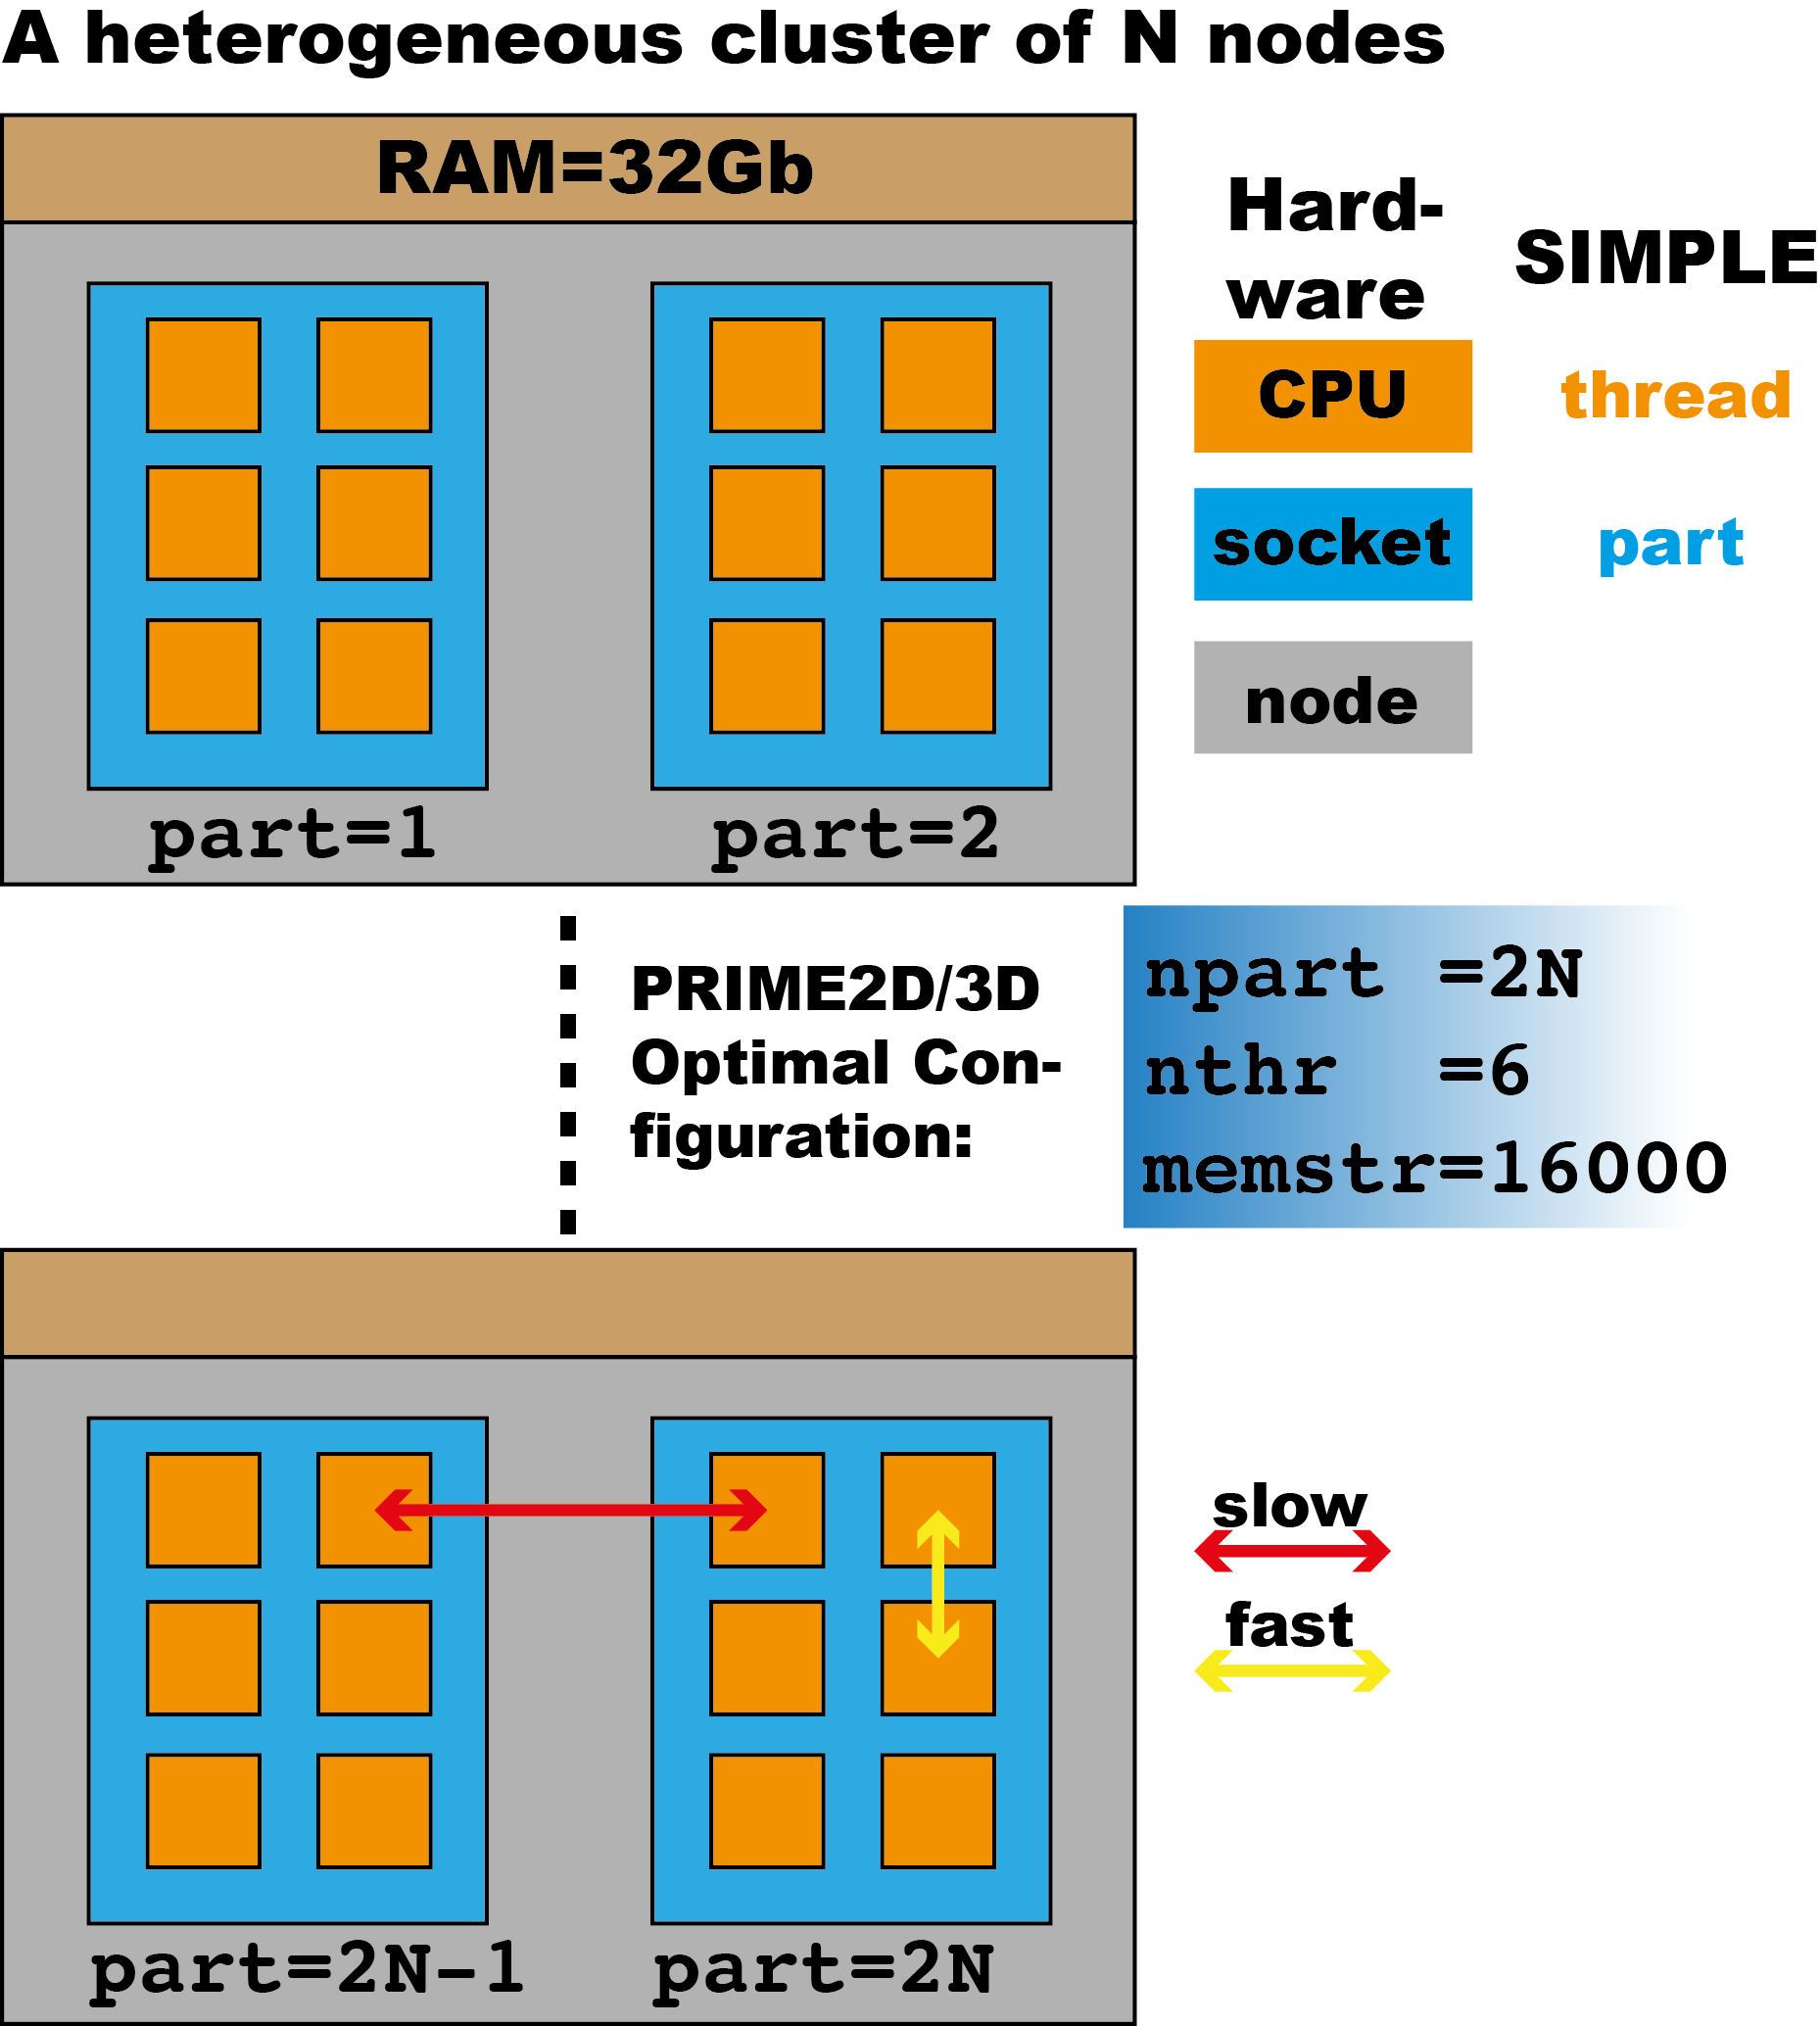
\includegraphics[keepaspectratio=true,scale=0.6]{./CPU_topo/cputopo}
\caption{\textbf{Configuration of the parallel PRIME-2D/3D execution on a heterogeneous cluster.} We here represent the nodes in  a heterogeneous cluster by two sockets with six CPUs each and 32Gb RAM/node. The best performance of PRIME--2D/3D is going to be obtained by partitioning  the jobs into \texttt{npart=2N} partitions, where \texttt{N} is the number of nodes. Each partition will then execute six threads \texttt{nthr=6} and these six threads will get access to half the RAM on the node (\texttt{memstr=16000}) because we have two sockets per node that need to share the RAM between them}
\end{SCfigure}
\\Every cluster is equipped with a job scheduler/workload manager that needs to be configured. The two most common job schedulers are SLURM (Simple Linux Utility for Resource Management) and PBS (Portable Batch System). We prefer SLURM, since it is a more modern and versatile job scheduler than PBS. All the instructions that need to be provided to the job scheduler have been separated out and put in the perl configuration module \texttt{scripts/simple\_clusterSpecs.pm}. A typical SLURM configuration is defined as
\begin{verbatim}
    ####################################################################
    # DEFINES DISTRIBUTED EXECUTION ON MYCLUSTER                       #
    ####################################################################
    our%MYCLUSTER_DISTR_ENV;
    $MYCLUSTER_DISTR_ENV{'SUBMITCMD'}='sbatch';
    $MYCLUSTER_DISTR_ENV{'SCRIPT'}="#!/bin/bash
    #SBATCH --mail-user=<<<<EMAIL>>>>
    #SBATCH --mail-type=FAIL
    #SBATCH --job-name=$NAME_DISTR
    #SBATCH --ntasks=1
    #SBATCH --ntasks-per-socket=1
    #SBATCH --cpus-per-task=<<<NTHR>>>
    #SBATCH --mem=<<<MEMSTR>>>
    #SBATCH --time=0-<<<HOURS>>>:<<<MINUTES>>>:0
    #SBATCH --output=outfile.%j
    #SBATCH --error=errfile.%j
    cd <<<EXECDIR>>> 
    <<<CMDSTRING>>> fromp=<<<START>>> top=<<<STOP>>> part=<<<PART>>>&
    &nthr=<<<NTHR>>> outfile=$ALGNDOC_FBODY<<<PART>>>.txt > OUT<<<PART>>>\nexit\n";
    $MYCLUSTER_DISTR_ENV{'SHMEMSCRIPT'}="#!/bin/bash
    #SBATCH --mail-user=<<<<EMAIL>>>>
    #SBATCH --mail-type=FAIL
    #SBATCH --job-name=$NAME_SHMEM_DISTR
    #SBATCH --ntasks=1
    #SBATCH --ntasks-per-socket=1
    #SBATCH --cpus-per-task=<<<NTHR>>>
    #SBATCH --mem=<<<MEMSTR>>>
    #SBATCH --time=0-<<<HOURS>>>:<<<MINUTES>>>:0
    #SBATCH --output=shmemoutfile.%j
    #SBATCH --error=shmemerrfile.%j
    cd <<<EXECDIR>>> 
    <<<CMDSTRING>>> nthr=<<<NTHR>>> > SHMEMJOBOUT\nexit\n";
\end{verbatim}
The \texttt{\&} character denotes a line break and the substitution tags
\begin{verbatim}
    <<<MYVARIABLE>>>
\end{verbatim}
describe variables that will be automatically substituted into the scripts. The variables \texttt{\$NAME\_DISTR} and \texttt{\$NAME\_SHMEM\_DISTR} are local to the module and describe the hardcoded names of the distribution scripts. In order to make the newly defined distributed environment accessible to SIMPLE we need to export it by adding it to the export array in the header of the module, so that the line
\begin{verbatim}
    @EXPORT = qw($ALGNDOC_FBODY %LOCAL_DISTR_ENV %MASSIVE_DISTR_ENV&
    &%MASSIVE2_DISTR_ENV %MONARCH_DISTR_ENV %OXFORD_DISTR_ENV&
    &%OXFORD2_DISTR_ENV %OXFORD3_DISTR_ENV  $CVL_DISTR_ENV);
\end{verbatim}
is updated to
\begin{verbatim}
    @EXPORT = qw($ALGNDOC_FBODY %LOCAL_DISTR_ENV %MASSIVE_DISTR_ENV&
    &%MASSIVE2_DISTR_ENV %MONARCH_DISTR_ENV %OXFORD_DISTR_ENV&
    &%OXFORD2_DISTR_ENV %OXFORD3_DISTR_ENV  $CVL_DISTR_ENV)&
    &%MYCLUSTER_DISTR_ENV;
\end{verbatim}
There are different versions of SLURM and PBS and different clusters may use different conventions for how to construct the script headers. For example on our \texttt{MASSIVE2} cluster we need to add to the headers
\begin{verbatim}
    #SBATCH --partition=cryoem
    #SBATCH --qos=vip_m2
\end{verbatim}
to indicate that we will use our dedicated \texttt{cryoem} partition and our dedicated queue \texttt{vip\_m2}. In \texttt{simple\_clusterSpecs.pm} there is also a template available for PBS
\begin{verbatim}
    ####################################################################
    # DEFINES DISTRIBUTED EXECUTION ON THE MASSIVE 1 CLUSTER           #
    ####################################################################
    our%MASSIVE_DISTR_ENV;
    $MASSIVE_DISTR_ENV{'SUBMITCMD'}='qsub';
    $MASSIVE_DISTR_ENV{'SCRIPT'}="#!/bin/bash
    #PBS -N $NAME_DISTR
    #PBS -l nodes=1:ppn=<<<NTHR>>>,mem=<<<MEMSTR>>>
    #PBS -l walltime=<<<HOURS>>>:<<<MINUTES>>>:0
    #PBS -o outfile.\$PBS_JOBID
    #PBS -e errfile.\$PBS_JOBID
    cd <<<EXECDIR>>> 
    <<<CMDSTRING>>> fromp=<<<START>>> top=<<<STOP>>> part=<<<PART>>>&
    &nthr=<<<NTHR>>> outfile=$ALGNDOC_FBODY<<<PART>>>.txt > OUT<<<PART>>>\nexit\n";
    $MASSIVE_DISTR_ENV{'SHMEMSCRIPT'}="#!/bin/bash
    #PBS -N $NAME_SHMEM_DISTR
    #PBS -l nodes=1:ppn=<<<NTHR>>>,mem=<<<MEMSTR>>>
    #PBS -l walltime=<<<HOURS>>>:<<<MINUTES>>>:0
    #PBS -o outfile.\$PBS_JOBID
    #PBS -e errfile.\$PBS_JOBID
    cd <<<EXECDIR>>> 
    <<<CMDSTRING>>> nthr=<<<NTHR>>> > SHMEMJOBOUT\nexit\n";
\end{verbatim}
but PBS does not provide any means to bind a set of threads to a particular socket. However, by utilising the \texttt{mpirun} command we can enforce this desired behaviour as exemplified below
\begin{verbatim}
    ####################################################################
    # DEFINES DISTRIBUTED EXECUTION ON SUSANS CLUSTER IN OXFORD        #
    ####################################################################
    our%OXFORD_DISTR_ENV;
    $OXFORD_DISTR_ENV{'SUBMITCMD'}='qsub';
    $OXFORD_DISTR_ENV{'SCRIPT'}="#!/bin/bash
    #PBS -N $NAME_DISTR
    #PBS -l nodes=1:ppn=<<<NTHR>>>,mem=<<<MEMSTR>>>
    #PBS -l walltime=<<<HOURS>>>:<<<MINUTES>>>:0
    #PBS -o outfile.\$PBS_JOBID
    #PBS -e errfile.\$PBS_JOBID
    #PBS -V
    #PBS -l naccesspolicy=UNIQUEUSER
    cd <<<EXECDIR>>> 
    mpirun -np 1 --bind-to-socket --cpus-per-proc <<<NTHR>>> <<<CMDSTRING>>>&
    &fromp=<<<START>>> top=<<<STOP>>> part=<<<PART>>> nthr=<<<NTHR>>>&
    &outfile=$ALGNDOC_FBODY<<<PART>>>.txt > OUT<<<PART>>>\nexit\n";
    $OXFORD_DISTR_ENV{'SHMEMSCRIPT'}="#!/bin/bash
    #PBS -N $NAME_SHMEM_DISTR
    #PBS -l nodes=1:ppn=<<<NTHR>>>,mem=<<<MEMSTR>>>
    #PBS -l walltime=<<<HOURS>>>:<<<MINUTES>>>:0
    #PBS -o outfile.\$PBS_JOBID
    #PBS -e errfile.\$PBS_JOBID
    #PBS -V
    #PBS -l naccesspolicy=UNIQUEUSER
    cd <<<EXECDIR>>> 
    mpirun -np 1 --bind-to-socket --cpus-per-proc <<<NTHR>>> <<<CMDSTRING>>>&
    &nthr=<<<NTHR>>> > SHMEMJOBOUT\nexit\n";
\end{verbatim}
Once our environment for distributed execution is established we use the {Program: \prgname{distr\_simple.pl}}, which supports distributed execution of the programs:
\begin{verbatim}
    simple_prime2D
    simple_prime3D
    simple_eo_recvol
    simple_recvol
    simple_simemimgs
\end{verbatim}
We normally let \prgname{distr\_simple.pl} run in the background on the login node of our cluster. We will discuss the execution routes in more detail in the \texttt{Workflows} section but an example of how to distribute \prgname{simple\_prime2D} using ten nodes is provided below. In order to reduce I/O latency we split the CTF phase-flipped image stack into as many partitions (\texttt{npart}) as we plan to execute
\begin{verbatim}
     $ simple_stackops stk=my_phaseflipped_ptcls.mrc split=npart
\end{verbatim}
Then, we are ready to execute in distributed mode
\begin{verbatim}
     $ nohup distr_simple.pl prg=prime2D npart=10 stk=ptcls.mrc smpd=1.77 msk=100
     ncls=600 refs=startcavgsmsk.mrc oritab=prime2D_startdoc.txt >> PRIME2DOUT &
\end{verbatim}
Another option available on clusters that use the SLURM scheduler is to use the \texttt{srun} command for \prgname{distr\_simple.pl} via
\begin{verbatim}
    $ srun --ntasks=1 --ntasks-per-socket=1 --cpus-per-task=1 --mem=200 --time=2-0:0:0
    --output=PRIME2DOUT.%j --error=PRIME2DERR.%j distr_simple.pl prg=prime2D 
    npart=10 stk=ptcls.mrc smpd=1.77 msk=100 ncls=600 refs=startcavgsmsk.mrc 
    oritab=prime2D_startdoc.txt &
\end{verbatim}
However, beta testers have reported that srun job sometimes dies with no warning, possibly because of the low tolerance for network errors. A more robust route may be to use \texttt{sbatch} as follows
\begin{verbatim}
    $ sbatch -p MYCLUSTER --wrap="distr_simple.pl prg=prime2D npart=10 stk=ptcls.mrc
    smpd=1.77 msk=100 ncls=600 refs=startcavgsmsk.mrc oritab=prime2D_startdoc.txt 
    >> PRIME2DOUT"
\end{verbatim}
where the \texttt{--wrap} flag automatically generates a bash script for the given command.

\subsection{CTF phase flipping}
\label{ctfflip}
SIMPLE uses the same CTF convention as CTFFIND\citep{Mindell:2003aa} and Frealign\citep{Grigorieff:2007aa} with the exception that defocus values are inputted in microns rather than Angstroms. The astigmatism angles are in units of degree. If you have a particle stack of uncorrected windowed single-particle images and you wish to multiply them with the sign of the CTF (phase flipping), please create a text file looking like
\begin{verbatim}
    dfx=2.56 dfy=2.76 angast=30.5
    dfx=3.50 dfy=3.33 angast=60.0
    dfx=1.98 dfy=2.02 angast=120.5
    ...
\end{verbatim}
with the same number of lines as the number of images in the stack, so that there is a one-to-one correspondence between each line of CTF parameters in the text file and each particle image in the stack. Now, use the program \prgname{simple\_stackops} to phase flip the stack
\begin{verbatim}
    $ simple_stackops stk=ptcls.mrc smpd=2 deftab=ctfparams.txt 
    ctf=flip kv=300 cs=2.7 fraca=0.07 outstk=ptcls_phflip.mrc
\end{verbatim}
and use the corrected stack \texttt{ptcls\_phflip.mrc} as input for the remaining workflows. Save the \texttt{ctfparams.txt} file somewhere safe, you might need it for future Wiener restoration in the refinement.

\subsection{2D alignment/clustering with PRIME2D}
\label{prime2D}
\begin{wrapfigure}{l}{0.4\textwidth}
\includegraphics[keepaspectratio=true,scale=0.3]{./PRIME2D_wflows/wflows}
\caption{PRIME-2D workflows}
\end{wrapfigure}
We provide a solver for the problem of simultaneous alignment and clustering of cryo-EM images (SAC) implemented in the program \prgname{simple\_prime2D}. It is assumed that you have a SPIDER or MRC stack of phase flipped particle images (see section \ref{ctfflip} above). The flowcharts of the workflows involving \prgname{simple\_prime2D} are depicted in Figure 2. There are two modes of execution: plain "2D alignment/clustering", assuming that you have a clean and nice data set with not too much junk, such as ice contaminations or particle aggregations. You begin executing \prgname{simple\_prime2D\_init} to produce the files \texttt{startcavgsmsk.mrc} and \texttt{prime2D\_startdoc.txt} containing the random references and random clustering solution. These files are are next used as input to \prgname{simple\_prime2D}. However, if you are planning on executing SIMPLE on a multi-socket workstation or cluster using \prgname{distr\_simple.pl} you have to split the stack into as many partitions (nodes) you are planning to run your job on. This step is necessary for reducing I/O latency. On single-socket machines it is not necessary to split the stack. Next, the generated files are inputted to \prgname{simple\_prime2D} together with the particle stack and a few control parameters, such as sampling distance (\texttt{smpd}), mask radius in pixels (\texttt{msk}), number of desired clusters (\texttt{ncls}) and low-pass limit (\texttt{lp}). The default low-pass limit is set to \texttt{lp=20 \AA{}} which ought to be suitable for all particles with a molecular weight above 300 kDa. You may have to include higher frequency components to obtain a good clustering solution for smaller molecules but beware of the problem of overfitting. If too much high-frequency information is included in the search, the solution obtained may be dominated by noise.

We also provide a "cleanup" workflow for processing of more challenging data sets. Perhaps your particles were automatically boxed and the stack includes a lot of false positives, such as ice contaminations, particle aggregations, hole edges etc. The first part of the "cleanup" workflow is identical to the original workflow. Next, the final class averages obtained with the first pass of clustering are ranked according to decreasing population with \prgname{simple\_rank\_cavgs} and a GUI (we use EMAN\citep{Ludtke:1999aa,Tang:2007aa}) is used to remove unwanted class averages. The program \prgname{simple\_map2ptcls} is then applied to map your manual selection of class averages back to the particle images. The selection is communicated via a text document named \texttt{mapped\_ptcls\_params.txt} by default. Every particle image receives a state assignment of one by default (\texttt{state=1}) and the particles corresponding to deleted class averages are assigned a state label of zero (\texttt{state=0}) in the outputted document. This prevents them from being considered in future processing steps. In order to obtain a "clean" clustering solution, execute the original workflow again but now inputting the \texttt{mapped\_ptcls\_params.txt} document to the \prgname{simple\_prime2D\_init} initialiser in order to propagate the selection. 

\subsection{\textit{Ab initio} 3D reconstruction with PRIME3D}
\label{prime3D}
\begin{wrapfigure}{l}{0.4\textwidth}
\includegraphics[keepaspectratio=true,scale=0.4]{./PRIME3D_wflows/abinitio_wflow}
\caption{PRIME-3D \textit{ab initio} workflow}
\end{wrapfigure}
We provide an \textit{ab initio 3D} reconstruction algorithm that operates either on class averages or on individual particle images. For small data sets (<10,000) images it is usually a better idea to skip the 2D alignment/clustering step and go directly to PRIME3D. For larger data sets or data sets with a lot of contaminations, such as ice, particle aggregations etc. we advice running PRIME2D first in "cleanup" mode and calculating an \textit{ab initio} map from "clean" class averages. The 3D PRIME algorithm is implemented in the program \prgname{simple\_prime3D}. It is assumed that you have a SPIDER or MRC stack of class averages (see section \ref{prime2D}) or phase flipped particle images (see section \ref{ctfflip}). The flowchart for the PRIME3D \textit{ab initio} reconstruction workflow is depicted in Figure 3. You begin executing \prgname{simple\_prime3D\_init} to produce the files \texttt{startvol\_state1.mrc} and \texttt{prime3D\_startdoc.txt} containing the initial random reference and the orientations used to obtain it. These files are are next used as input to \prgname{simple\_prime3D}. However, if you are planning on executing SIMPLE on a multi-socket workstation or cluster using \prgname{distr\_simple.pl} you have to split the stack into as many partitions (nodes) you are planning to run your job on. This step is necessary for reducing I/O latency. On single-socket machines it is not necessary to split the stack. Next, the generated files are inputted to \prgname{simple\_prime3D} together with the particle stack and a few control parameters, such as sampling distance (\texttt{smpd}) and mask radius in pixels (\texttt{msk}). Details about how to run PRIME3D and how the initial low-pass limit is set and how it is updated throughout a PRIME3D run is described in the \prgname{simple\_prime3D} section, below. To check the automatically determined low-pass limit range, use the \prgname{simple\_resrange} program.

\subsection{Worked-out example on GroEL}

To further illustrate how to use the SIMPLE suite of programs, we provide the following comprehensive worked-out example, including all commands executed when reconstructing the D7 symmetric GroEL chaperonin. The same workflow was used to process a series of experimental datasets with high, low or no symmetry, described in our recent paper \citep{reboul2016stochastic}. The workflow consists of four major steps
\begin{enumerate}
\item 2D alignment and clustering of the images using \prgname{simple\_prime2D}
\item asymmetric 3D reconstruction from the class averages using \prgname{simple\_prime3D}
\item symmetrisation of the volume using \prgname{simple\_symsrch}
\item refinement of the symmetrised volume using \prgname{simple\_prime3D}
\end{enumerate}
The data set consisted of 10,000 phase flipped images with 140x140 pixels dimension, randomly selected from a larger publicly available data set \citep{Stagg:2008aa}. Throughout the different steps of the workflow we used a a circular mask radius of \texttt{msk=60} pixels and sampling distance of \texttt{smpd=1.62}.

\subsubsection{2D alignment and clustering of the images}
\label{2dclust}

Prior to 2D alignment and clustering, we begin by minimising the effect that off-centre particles could have on the subsequent steps. The method is not aimed at determining the rotational origin shifts exactly but only to roughly centre the particles in the box. This is done by bringing all particle images into broad register with respect to their 2D shifts only, regardless of their in-plane rotation. \prgname{simple\_stackops} with the argument \texttt{shalgn=yes} is used, providing our stack (\texttt{stk=particles.spi}), sampling distance (\texttt{smpd=1.62}) and mask radius in pixels (\texttt{msk=60} as input
\begin{verbatim}
    $ simple_stackops stk=particles.spi smpd=1.62 msk=60 
    shalgn=yes trs=3.5 lp=20 nthr=8 outstk=particles_sh.spi
\end{verbatim}
The shift alignment is done with a hard low-pass limit of 20 \AA{} (\texttt{lp=20}), as are most of the following steps. The iterative process will typically take a dozen iterations (a few minutes). The \texttt{trs} argument limits the shift search to the $[-trs,trs]$ range. We typically set the \texttt{trs} argument to 2.5\% of the image dimension (140). There are 8 CPUs on our machine so we set the number of threads \texttt{nthr=8}. A new centred stack (named according to the \texttt{outstk} argument) will be written to disk and we will use this one for the reminder of the workflow. A document named \texttt{shiftdoc.txt} by default that contains the calculated shifts is also created.

Next we generate random class averages to initiate the 2D clustering procedure. Given the modest size of our dataset (10,000 images) we choose \texttt{ncls=200} to obtain sufficiently populated classes. We recommended increasing this number to at least 500 for larger datasets (>30,000 images).
\begin{verbatim}
    $ simple_prime2D_init stk=particles_sh.spi smpd=1.62 msk=60 ncls=200 nthr=8
\end{verbatim}
\prgname{simple\_prime2D\_init} will rapidly generate evenly populated class averages with random in-plane rotations. The stacks of 200 class averages are named \texttt{startcavgsmsk.spi} and \texttt{startcavgs.spi} (with and without mask). Next, we execute the 2D alignment and clustering in distributed mode
\begin{verbatim}
    $ simple_stackops stk=particles_sh.spi split=1
    $ nohup distr_simple.pl prg=prime2D stk=particles_sh.spi
    oritab=prime2D_startdoc.txt refs=startcavgsmsk.spi ncls=200
    srch_inpl=yes smpd=1.62 msk=60 lp=20 npart=1 > PRIME2DOUT &
\end{verbatim}
The first instruction prepares the split stack for distributed execution. In our case we ran the clustering on a Linux workstation with 1 CPU chipset so we simply set \texttt{split=1}. If your machine has two chipsets, set split to 2 but keep in mind that the \texttt{npart} argument in the following instruction also needs to be set to 2. The second instruction starts the actual 2D clustering using the randomised classes as a starting point (\texttt{refs} argument). It will take approximately 15 iterations and little under 2 hours on a modern workstation with 8 CPUs. In the last lines of the log file \texttt{PRIME2DOUT} you should see something looking like
\begin{verbatim}
    >>> DISTRIBUTION OVERLAP:                 0.9589
    >>> PERCENTAGE OF SEARCH SPACE SCANNED:  99.6
    >>> CORRELATION:                          0.7521
    >>> CONVERGED: .YES.
\end{verbatim}
Our criterion for convergence is based the stability of the clusters obtained. In other words, when the cluster assignments are nearly identical from one iteration to the next (distribution overlap  >95\% on average) and the particles cannot find a better matching average (fraction of search space scanned >99\%) the alignment and clustering stops. In addition, each run is structured as follows. Until near convergence (search space scanned <90\%) only cluster assignment and in-plane rotations are searched. After this, shifts are also searched and their limit is automatically set to 2.5\% of the image dimension (see above). Every iteration produces a folder named \texttt{prime2D\_round\_XX} that contains all the information to continue a run: a document with the current in-plane parameters (\texttt{prime2Ddoc\_XX.txt}) and two stacks of the current 200 class averages (masked and unmasked).

A number of temporary files are also created but they are only used internally and will be automatically deleted at the end of the run. As computer and network failures are part of using workstations and supercomputers you will be able to continue an interrupted run using the files present in these self-contained folders. You can also automatically remove the temporary files by simply typing: \prgname{prime\_cleanup.pl}. Never do this while the application is running.  It is also necessary to keep the current folder organised to avoid data loss and confusion. We do not need the split stack anymore, so type
\begin{verbatim}
    $ rm stack_part*.spi
\end{verbatim}
Visual examination of the 200 class averages (\texttt{prime2D\_round\_15/cavgs\_iter15.spi}) shows numerous images with distinctive features of GroEL such as the double ring structure and the heptameric C-symmetric rings on a uniform grey background. One can also note blurrier images with less contrast. Typically, these correspond to lowly populated classes where the weaker SNR is likely to contribute little to the subsequent 3D reconstruction. Consequently, we rank the class averages by decreasing order of their population
\begin{verbatim}
    $ simple_rank_cavgs stk=prime2D_round_15/cavgs_iter15.spi 
    oritab=prime2D_round_15/prime2Ddoc_15.txt outstk=ranked_cavgs.spi
\end{verbatim}
After visual inspection of the ranked class averages (we use EMAN for this \citep{Ludtke:1999aa,Tang:2007aa}) we decide to discard the noisier/blurrier images by keeping the first 160 averages in the ranked stack. This discards clusters containing less than 30 images per class. We simply extract the top 160 averages using the command
\begin{verbatim}
    $ simple_stackops stk=ranked_cavgs.spi fromp=1 top=160 outstk=selected_cavgs.spi
\end{verbatim}
where \texttt{fromp} and \texttt{top} define the range of images to keep. With this reduced stack (\texttt{selected\_cavgs.spi}) we will generate an \textit{ab initio} 3D reconstruction of the molecule using \prgname{simple\_prime3D}

\subsubsection{\textit{Ab initio} 3D reconstruction}

We first need a random volume to initiate the search of the five in-plane and out-of-plane parameters of our selected class averages. As in the previous 2D analysis, we execute
\begin{verbatim}
    $ simple_prime3D_init stk=selected_cavgs.spi smpd=1.62 msk=60 nthr=8 lp=20
\end{verbatim}
Consistently with section \ref{2dclust}, we use a low-pass limit of 20 \AA{} (\texttt{lp=20}). This command will generate two files: a volume reconstructed from random orientation parameters (\texttt{startvol\_state1.spi}) and the document containing these parameters (\texttt{prime3D\_startdoc.txt}). We start the search with
\begin{verbatim}
    $ simple_stackops stk=selected_cavgs.spi split=1
    $ nohup distr_simple.pl prg=prime3D stk=selected_cavgs.spi 
    vol1=startvol_state1.spi smpd=1.62 msk=60 lp=20 
    oritab=prime3D_startdoc.txt npart=1 > PRIME3DOUT &
\end{verbatim}
Again, we first split the stack for distributed execution. Then, we run PRIME3D providing the randomised orientations (\texttt{oritab} argument) and volume (\texttt{vol1} argument) that we have just prepared. After approximately 16 iterations the run converges. At the end of PRIME3DOUT you will find
\begin{verbatim}
    >>> ANGLE OF FEASIBLE REGION:            14.1
    >>> AVERAGE ANGULAR DISTANCE BTW ORIS:    2.4 
    >>> PERCENTAGE OF SEARCH SPACE SCANNED: 100.0
    >>> CORRELATION:                          0.9178
    >>> ANGULAR SDEV OF MODEL:               40.81
    >>> UPDATE LOW-PASS LIMIT: .NO.
    >>> CONVERGED: .YES.
\end{verbatim}
The \texttt{recvol\_state1.spi} volume and the corresponding orientation parameters (\texttt{prime3Ddoc\_16.txt}) are produced in the \texttt{prime3D\_round\_16} folder. The volume is blobby but still captures the overall shape of GroEL. Keep in mind that we have so far made no assumption about symmetry and the volume has been reconstructed in the C1 symmetry group.

\subsubsection{Symmetrisation of the volume}

In order to symmetrise the volume, we need to identify the principal axis of symmetry given the known D7 point-group symmetry group of GroEL. This is done with \prgname{simple\_symsrch}, given the C1 volume and orientation parameters (\texttt{vol1} and \texttt{oritab}) and using the same low-pass limit as previously (\texttt{lp=20}). The symmetrised orientations are outputted in the text file \texttt{sym\_d7.txt} (\texttt{outfile} argument). We identify the principal symmetry axis of the volume by executing 
\begin{verbatim}
    $ simple_symsrch vol1=prime3D_round_16/recvol_state1.spi smpd=1.62 msk=60 
    oritab=prime3D_round_16/prime3Ddoc_16.txt pgrp=d7 outfile=sym_d7.txt nthr=8 
    lp=20 > SYMOUT
\end{verbatim}
The program prints the identified symmetry axis
\begin{verbatim}
    >>> FOUND SYMMETRY AXIS ORIENTATION:
    e1=276.596588 e2=80.9958649 e3=297.840454 x=0.00000000 y=0.00000000 
    mi=0.00000000 mi_hard=0.00000000 dist=180.000000 state=1.00000000 
    corr=0.787599325 w=1.00000000 class=1.00000000 mirr=0.00000000 frac=0.00000000
\end{verbatim}
and we use \prgname{simple\_eo\_recvol} to reconstruct a symmetrised volume
\begin{verbatim}
    $ simple_eo_recvol stk=selected_cavgs.spi 
    oritab=sym_d7.txt smpd=1.62 msk=60 nthr=8 pgrp=d7
\end{verbatim}
Output is the optimal principal axis of symmetry (\texttt{e1}, \texttt{e2} and \texttt{e3} are the phi,theta and psi angles) along with its correlation (\texttt{corr}). It is likely that you will obtain different values for the axis of symmetry upon different runs. This is because of the stochastic nature of the 2D/3D analyses, which cause the 3D reconstruction to be arbitrarily oriented with respect to the principal symmetry axis. Nonetheless, the final volume is reproducible and captures the structure of GroEL as judged by the numerous existing crystallographic and EM structures.

With the new symmetrised orientation parameters of the class averages we now want to map this information back to the individual particle images. To do this we first create a text file called \texttt{doclist.txt} that contains a single line
\begin{verbatim}
    $ ls -1 sym_d7.txt > doclist.txt
\end{verbatim}
and then map the orientation parameters of the class averages to the particles (\texttt{stk}) by providing the selected class averages (\texttt{stk2}), all the original class averages (\texttt{stk3}) and the in-plane parameters obtained in the first \prgname{simple\_prime2D} run (\texttt{oritab}) to the program \prgname{simple\_map2ptcls}
\begin{verbatim}
    $ simple_map2ptcls stk=particles_sh.spi stk2=selected_cavgs.spi 
    stk3=cavgs_iter16.spi oritab=prime2D_round_16/prime2Ddoc_16.txt 
    doclist=doclist.txt nthr=8
\end{verbatim}
Next we reconstruct a symmetrised volume from the particles using the mapped orientation parameters (called \texttt{mapped\_ptcls\_params.txt} by default) and specifying the symmetry group (\texttt{pgrp=d7})
\begin{verbatim}
    $ simple_eo_recvol stk=particles_sh.spi oritab=mapped_ptcls_params.txt 
    smpd=1.62 msk=60 nthr=8 pgrp=d7
\end{verbatim}
After several minutes we obtain a new volume (\texttt{recvol\_state1msk.spi}) and its resolution
\begin{verbatim}
    >>> RESOLUTION AT FSC=0.143 DETERMINED TO:  12.60
    >>> RESOLUTION AT FSC=0.500 DETERMINED TO:  17.45
\end{verbatim}
As \texttt{recvol\_state1msk.spi} is the default name used internally by \prgname{simple\_prime3D} it is best to rename it to avoid having it overwritten
\begin{verbatim}
    $ mv recvol_state1msk.spi sym_recvol_state1msk.spi
\end{verbatim}
\prgname{simple\_eo\_recvol} and \prgname{simple\_prime3D} also produce a file \texttt{fsc\_state1.bin} that contains the FSC plot. Make sure to backup this file as  \prgname{simple\_prime3D} will overwrite it if executed in the same folder. Here we just copy it because in the next step we will refine the volume and  \prgname{simple\_prime3D}  will require the information contained in \texttt{fsc\_state1.bin} to initiate the refinement
\begin{verbatim}
    $ cp fsc_state1.bin eo_fsc_state1.bin
\end{verbatim}

\subsubsection{Refinement of the symmetrised volume using \prgname{simple\_prime3D}}

Finally, we refine our initial model while applying D7 symmetry with  \prgname{simple\_prime3D}
\begin{verbatim}
    $ simple_stackops stk=particles_sh.mrc split=8
    $ nohup distr_simple.pl prg=prime3D stk=groel-stk.spi
    vol1=sym_recvol_state1msk.spi smpd=1.62 msk=60 
    eo=yes oritab=mapped_ptcls_params.txt npart=8 > 
    PRIME3DOUT2 &
\end{verbatim}
With the first instruction we split the stack for distributed execution. Here the refinement run will be split over 8 different CPU sockets on a Linux cluster (\texttt{split=8}; see Section \ref{paraexec} for more details). We use PRIME3D differently this time. Instead of setting a 20 \AA{} low-pass limit, the resolution of the volume is calculated automatically at every iteration (\texttt{eo=yes}) and we are starting from our symmetrised volume (\texttt{vol1=sym\_recvol\_state1msk.spi}). After the 10 iterations required for convergence, the final resolution  (better than 8 \AA{}) is printed in the end of the \texttt{PRIME3DOUT2} output (and also stored in the \texttt{fsc\_state1.bin}). Examination of the volume shows helical features consistent with the GroEL X-ray structure.
\begin{verbatim}
    >>> RESOLUTION AT FSC=0.143 DETERMINED TO:   7.32
    >>> RESOLUTION AT FSC=0.500 DETERMINED TO:   8.10
\end{verbatim}
\textbf{A note on overfitting:} In contrast to most other packages, the only exception being Frealign, SIMPLE does all of its interpolations and correlation calculations in the Fourier domain. Other packages may argue that they do as well but there are subtle important differences. For example, Spider, EMAN and SPARX interpolate polar coordinates in real space and then calculate one-dimensional Fourier transforms along concentric rings to obtain their "polar Fourier transforms", which are in fact polar real images. The advantage of doing it in this way is that you can use a hard mask in real space and avoid including too much background noise in the representation. However, the fundamental disadvantage is that you loose the ability to control which Fourier components are being used for the matching. Initially, it was assumed that the low-pass filtering of the volume based on the FSC ought to be sufficient to avoid overfitting. This has proven not to be true with this kind of representation, as both EMAN2 and SPARX now implement the "gold-standard approach". We instead use gridding interpolation \textit{in Fourier space} to obtain our polar central sections. The minor disadvantage is that we have to apply a soft-edged mask in real space and risk introduce slightly more background noise in the representation. However, the major advantage is that we can control exactly which Fourier components we use for matching. The default high-pass limit is set to Fourier index 2 but if you think you have a lot of inelastic scattering at low resolution (this is typical for icosahedral viruses) you may want to change the high-pass limit via \texttt{hp=X \AA{}}. The hard low-pass limit, when \prgname{simple\_prime3D} is executed with \texttt{eo=yes} is set according to the \texttt{FSC=0.143} criterion. We have yet to detect any overfitting visually or using the noise substitution test \citep{Chen:2013aa} with this approach on standard EM data obtained with the underfocusing approach. However, while processing close-to-focus phase plate data we have observed severe overfitting and we recommend to battle it using hard low-pass limitation with \texttt{lpstop=X \AA{}}. If you do all your analyses with a hard  low-pass limit of \texttt{X} and the resolution extends significantly beyond the limit, there should be no reason to worry about overfitting.

\section{Command Line Dictionary}
\begin{tabular}{ll}
\texttt{acf}&{calculate autocorrelation function(yes|no)\{no\}}\\
\texttt{amsklp}&{low-pass limit for envelope mask/centering mask(in \AA{})}\\
\texttt{angerr}&{angular error(in degrees)\{0\}}\\
\texttt{append}&{append in context of files(yes|no)\{no\}}\\
\texttt{astigerr}&{astigmatism error(in microns)\{0.1\}}\\
\texttt{athres}&{angular threshold(in degrees)}\\
\texttt{automsk}&{envelope masking(yes|no)\{no\}}\\
\texttt{avg}&{calculate average(yes|no)}\\
\texttt{bfac}&{bfactor for sharpening/low-pass filtering(in \AA{}**2)\{200.\}}\\
\texttt{bfacerr}&{bfactor error in simulated images(in \AA{}**2)\{0\}}\\
\texttt{bin}&{binarise image(yes|no)\{no\}}\\
\texttt{binwidth}&{binary layers grown for molecular envelope(in pixels)\{1\}}\\
\texttt{box}&{square image size(in pixels)}\\
\texttt{boxconvsz}&{size of box used for box-convolution(in pixels)}\\
\texttt{boxtab}&{table (text file) of files with EMAN particle coordinates(*.txt/*.asc)}\\
\texttt{center}&{center image(s)(yes|no)\{no\}}\\
\texttt{chunksz}&{number of images/orientations in chunk}\\
\texttt{class}&{cluster identity of particle}\\
\texttt{clip}&{clipped image box size(in pixels)}\\
\texttt{clustvalid}&{validate clustering(yes|homo|no)\{no\}}\\
\texttt{comlindoc}&{shc\_clustering\_nclsX.txt}\\
\texttt{compare}&{do comparison(yes|no)\{no\}}\\
\texttt{corner}&{corner size(in pixels)\{0\}}\\
\texttt{countvox}&{count the number of voxels(yes|no)\{no\}}\\
\texttt{cs}&{spherical aberration constant(in mm)\{2.7\}}\\
\texttt{ctf}&{ctf flag(yes|no|flip)\{no\}}\\
\texttt{ctfsq}&{apply ctf**2 to the images(yes|no)\{no\}}\\
\texttt{ctfsqspec}&{filename of ctf**2 spectrum\{ctfsqspec\_state01.bin\}}\\
\texttt{ctfstats}&{calculate ctf statistics(yes|no)\{no\}}\\
\texttt{cube}&{side size(in pixels)\{0\}}\\
\texttt{deferr}&{defocus error(in microns)\{1.0\}}\\
\texttt{defocus}&{defocus(in microns)\{3.\}}\\
\texttt{deftab}&{text file with CTF info(*.txt/*.asc)}\\
\texttt{dir}&{move selected files to here\{selected\}}\\
\texttt{discrete}&{discrete(yes|no)\{no\}}\\
\texttt{doclist}&{list of oritabs for different states}\\
\texttt{dynlp}&{automatic resolution limit update(yes|no)\{yes\}}\\
\texttt{e1}&{1st Euler(in degrees)\{0\}}\\
\texttt{e2}&{2nd Euler(in degrees)\{0\}}\\
\texttt{e3}&{3d Euler(in degrees)\{0\}}\\
\texttt{edge}&{edge size for softening molecular envelope(in pixels)}\\
\texttt{endian}&{endiannesss of files(big|little|native)\{native\}}\\
\texttt{eo}&{use FSC for filtering and low-pass limit update(yes|no)\{no\}}\\
\texttt{errify}&{introduce error(yes|no)\{no\}}\\
\texttt{even}&{calculate even eo-pair(yes|no)\{no\}}\\
\texttt{fbody}&{file body}\\
\texttt{filetab}&{list of files(*.txt/*.asc files)}\\
\texttt{filwidth}&{width of filament (in \AA{})}\\
\texttt{find}&{Fourier index}\\
\texttt{fix\_gpu}&{fix GPU execution to one device(yes|no)\{no\}}\\
\texttt{fname}&{file name}\\
\texttt{frac}&{fraction of ptcls(0-1)\{1\}}\\
\texttt{fraca}&{fraction of amplitude contrast used for fitting CTF\{0.07\}}\\
\end{tabular}

\begin{tabular}{ll}
\texttt{fracdeadhot}&{fraction of dead or hot pixles\{0.01\}}\\
\texttt{frameavg}&{nr of frames to average\{0\}}\\
\texttt{fromf}&{start frame index}\\
\texttt{fromp}&{start ptcl index}\\
\texttt{fsc}&{binary file with FSC info\{fsc\_state01.bin\}}\\
\texttt{ft2img}&{convert Fourier transform to real image of power(yes|no)\{no\}}\\
\texttt{grow}&{number of binary layers to grow(in pixels)}\\
\texttt{guinier}&{calculate Guinier plot(yes|no)\{no\}}\\
\texttt{hfun}&{function used for normalization(sigm|tanh|lin)\{sigm\}}\\
\texttt{hist}&{give variable for histogram plot}\\
\texttt{hp}&{high-pass limit(in \AA{})}\\
\texttt{inner}&{inner mask radius(in pixels)}\\
\texttt{jumpsz}&{size of contigous segment}\\
\texttt{kv}&{acceleration voltage(in kV)\{300.\}}\\
\texttt{label}&{discrete label(class|state)\{class\}}\\
\texttt{lp}&{low-pass limit(in \AA{})}\\
\texttt{lpstart}&{start low-pass limit\{15\}}\\
\texttt{lpstop}&{stop low-pass limit\{8\}}\\
\texttt{mapnn}&{map nearest neighbors on micrograph(yes|no)\{no\}}\\
\texttt{masscen}&{center using binarisation and mass centering(yes|no)\{no\}}\\
\texttt{maxits}&{maximum number of iterations\{500\}}\\
\texttt{minp}&{minimum cluster population\{10\}}\\
\texttt{mirr}&{mirror(no|x|y)\{no\}}\\
\texttt{moldiam}&{molecular diameter(in \AA{})}\\
\texttt{msk}&{mask radius(in pixels)}\\
\texttt{mskfile}&{maskfile.ext}\\
\texttt{msktype}&{type of mask(hard|soft)\{soft\}}\\
\texttt{mul}&{origin shift multiplication factor\{1\}}\\
\texttt{mw}&{molecular weight(in kD)}\\
\texttt{ncls}&{nr of clusters}\\
\texttt{ndiscrete}&{nr of discrete orientations}\\
\texttt{ndocs}&{nr of documents}\\
\texttt{neg}&{invert contrast of images(yes|no)\{no\}}\\
\texttt{newbox}&{new box size(in pixels)}\\
\texttt{nframes}&{number of frames\{30\}}\\
\texttt{noise}&{noise initialisation(yes|no)\{no\}}\\
\texttt{noise\_norm}&{normalise based on sdev of background(yes|no)\{no\}}\\
\texttt{norec}&{do not reconstruct volume(s)(yes|no)\{no\}}\\
\texttt{norm}&{do statistical normalisation avg}\\
\texttt{npart}&{nr of partitions in distributed exection}\\
\texttt{npeaks}&{nr of nonzero orientation weights\{1\}}\\
\texttt{npix}&{number of pixles/voxels in binary representation}\\
\texttt{nptcls}&{nr of images in stk}\\
\texttt{nran}&{number of random images to select}\\
\texttt{nspace}&{nr of projection directions\{20\}}\\
\texttt{nstates}&{nr of states to reconstruct}\\
\texttt{nthr}&{nr of OpenMP threads\{1\}}\\
\texttt{numlen}&{length of number string}\\
\texttt{nvox}&{number of voxels\{0\}}\\
\texttt{odd}&{calculate odd eo-pair(yes|no)\{no\}}\\
\texttt{oritab}&{table (text file) of orientations(*.asc/*.txt)}\\
\texttt{oritab2}&{2nd table (text file) of orientations(*.asc/*.txt)}\\
\texttt{outer}&{outer mask radius(in pixels)}\\
\end{tabular}

\begin{tabular}{ll}
\texttt{outfile}&{output alignment document}\\
\texttt{outside}&{only extract boxes within the micrograph boundaries(yes|no)\{yes\}}\\
\texttt{outstk}&{output image stack\{outstk.ext\}}\\
\texttt{outvol}&{output volume\{outvol.ext\}}\\
\texttt{paramtab}&{per-micrograph parameters to transfer (CTF/movie shifts)}\\
\texttt{pgrp}&{point-group symmetry(cn|dn|t|o|i)\{c1\}}\\
\texttt{phrand}&{phase randomize(yes|no)\{no\}}\\
\texttt{plot}&{make plot(yes|no)\{no\}}\\
\texttt{prg}&{SIMPLE program to execute}\\
\texttt{pspecsz}&{size of power spectrum(in pixels)\{512\}}\\
\texttt{refine}&{refinement mode(no|shc|neigh|shcneigh|qcont|qcontneigh)\{no\}}\\
\texttt{refs}&{initial2Dreferences.ext}\\
\texttt{remap}&{adjust the number of clusters by splitting(yes|no)\{no\}}\\
\texttt{rnd}&{random(yes|no)\{no\}}\\
\texttt{scale}&{image scale factor\{1\}}\\
\texttt{set\_gpu}&{index of GPU device used(1-MAX\_N\_GPU)\{0\}}\\
\texttt{shalgn}&{do 2D shift alignment(yes|no)\{no\}}\\
\texttt{shbarrier}&{use shift search barrier constraint(yes|no)\{yes\}}\\
\texttt{shell\_norm}&{normalise based on power spectrum (yes|no)\{no\}}\\
\texttt{sherr}&{shift error(in pixels)\{2\}}\\
\texttt{shrink}&{shrink factor\{1\}}\\
\texttt{single}&{simulate a single image(yes|no)\{no\}}\\
\texttt{smpd}&{sampling distance, same as EMANs apix(in \AA{})}\\
\texttt{snr}&{signal-to-noise ratio}\\
\texttt{soften}&{soften envelope with cosine edge(yes|no)\{no\}}\\
\texttt{speckind}&{power spectrum kind(amp|square|phase|real|log|sqrt)\{sqrt\}}\\
\texttt{split}&{nr of partitions to split the stack into}\\
\texttt{srch\_inpl}&{search in-plane degrees of freedom(yes|no)\{yes\}}\\
\texttt{startit}&{start iterating from here}\\
\texttt{state}&{state to extract}\\
\texttt{state2split}&{state group to split}\\
\texttt{stats}&{provide statistics(yes|no)\{yes\}}\\
\texttt{stk}&{particle stack with all images(ptcls.ext)}\\
\texttt{stk2}&{2nd stack(in map2ptcls/select: selected(cavgs).ext)}\\
\texttt{stk3}&{3d stack (in map2ptcls/select: (cavgs)2selectfrom.ext)}\\
\texttt{thres}&{threshold for binarisation(0-1)}\\
\texttt{tof}&{stop frame index}\\
\texttt{top}&{stop particle index}\\
\texttt{trs}&{maximum halfwidth shift(in pixels)}\\
\texttt{trsstats}&{provide origin shift statistics(yes|no)\{no\}}\\
\texttt{use\_gpu}&{execute SIMPLE on GPU(yes|no)\{no\}}\\
\texttt{vis}&{visualise(yes|no)}\\
\texttt{vol1}&{input volume no1(invol1.ext)}\\
\texttt{vol2}&{input volume no2(invol2.ext)}\\
\texttt{vollist}&{table (text file) of volume files(*.txt/*.asc)}\\
\texttt{voltab}&{table (text file) of volume files(*.txt/*.asc)}\\
\texttt{voltab2}&{2nd table (text file) of volume files(*.txt/*.asc)}\\
\texttt{which\_iter}&{iteration nr}\\
\texttt{width}&{falloff of inner mask(in pixels)\{10\}}\\
\texttt{xdim}&{x dimension(in pixles)}\\
\texttt{xfel}&{images are XFEL diffraction patterns(yes|no)\{no\}}\\
\texttt{xsh}&{x shift(in pixels)\{0\}}\\
\texttt{ydim}&{y dimension(in pixles)}\\
\end{tabular}

\begin{tabular}{ll}
\texttt{ysh}&{y shift(in pixels)\{0\}}\\
\texttt{zero}&{zeroing(yes|no)\{no\}}\\
\texttt{zsh}&{z shift(in pixels)\{0\}}\\
\end{tabular}

\section{Individual SIMPLE programs}

\subsection{Simulator programs}

\subsubsection{Program: \prgname{simimgs}}
\label{simimgs}
\prgname{simimgs} is a program for simulating cryo-EM images. It is not a very sophisticated simulator, but it is nevertheless useful for testing purposes. It does not do any multi-slice simulation and it cannot be used for simulating molecules containing heavy atoms. It does not even accept a PDB file as an input. Input is a cryo-EM map, which we usually generate from a PDB file using EMAN's program pdb2mrc. simimgs then projects the volume using Fourier interpolation, applies 20\% of the total noise to the images (pink noise), Fourier transforms them, and multiplies them with astigmatic CTF and B-factor. The images are inverse FTed before the remaining 80\% of the noise (white noise) is added.

\begin{verbatim}
USAGE:
bash-3.2$ simple_exec prg=simple_program key1=val1 key2=val2 ...

REQUIRED
vol1   = input volume no1(invol1.ext)
smpd   = sampling distance, same as EMANs apix(in A)
msk    = mask radius(in pixels)
nptcls = nr of images in stk
snr    = signal-to-noise ratio

OPTIONAL
nthr      = nr of OpenMP threads{1}
sherr     = shift error(in pixels){2}
oritab    = table (text file) of orientations(*.asc/*.txt)
outfile   = output alignment document
outstk    = output image stack{outstk.ext}
single    = simulate a single image(yes|no){no}
ndiscrete = nr of discrete orientations
ctf       = ctf flag(yes|no|flip){no}
kv        = acceleration voltage(in kV){300.}
cs        = spherical aberration constant(in mm){2.7}
fraca     = fraction of amplitude contrast used for fitting CTF{0.07}
deftab    = text file with CTF info(*.txt/*.asc)
defocus   = defocus(in microns){3.}
deferr    = defocus error(in microns){1.0}
astigerr  = astigmatism error(in microns){0.1}
bfac      = bfactor for sharpening/low-pass filtering(in A**2){200.}
bfacerr   = bfactor error in simulated images(in A**2){0}
\end{verbatim}

\subsubsection{Program: \prgname{simmovie}}
\label{simmovie}
\prgname{simmovie} is a program for crude simulation of a DDD movie. Input is a set of projection images to place. Movie frames are then generated related by randomly shifting the base image and applying two different noise sources: shot and detector noise.

\begin{verbatim}
USAGE:
bash-3.2$ simple_exec prg=simple_program key1=val1 key2=val2 ...

REQUIRED
stk  = particle stack with all images(ptcls.ext)
smpd = sampling distance, same as EMANs apix(in A)
msk  = mask radius(in pixels)
xdim = x dimension(in pixles)
ydim = y dimension(in pixles)
snr  = signal-to-noise ratio

OPTIONAL
nthr    = nr of OpenMP threads{1}
nframes = number of frames{30}
trs     = maximum halfwidth shift(in pixels)
vis     = visualise(yes|no)
kv      = acceleration voltage(in kV){300.}
cs      = spherical aberration constant(in mm){2.7}
fraca   = fraction of amplitude contrast used for fitting CTF{0.07}
deftab  = text file with CTF info(*.txt/*.asc)
defocus = defocus(in microns){3.}
bfac    = bfactor for sharpening/low-pass filtering(in A**2){200.}
\end{verbatim}

\subsubsection{Program: \prgname{simsubtomo}}
\label{simsubtomo}
\prgname{simsubtomo} is a program for crude simulation of a subtomograms.

\begin{verbatim}
USAGE:
bash-3.2$ simple_exec prg=simple_program key1=val1 key2=val2 ...

REQUIRED
vol1   = input volume no1(invol1.ext)
smpd   = sampling distance, same as EMANs apix(in A)
nptcls = nr of images in stk
snr    = signal-to-noise ratio

OPTIONAL
nthr = nr of OpenMP threads{1}
\end{verbatim}

\subsection{Pre-processing programs}

\subsubsection{Program: \prgname{select\_frames}}
\label{select_frames}
\prgname{select\_frames} is a program for selecting contiguous segments of frames from DDD movies.

\begin{verbatim}
USAGE:
bash-3.2$ simple_exec prg=simple_program key1=val1 key2=val2 ...

REQUIRED
filetab = list of files(*.txt/*.asc files)
fbody   = file body
fromf   = start frame index
tof     = stop frame index
smpd    = sampling distance, same as EMANs apix(in A)

OPTIONAL
startit = start iterating from here
\end{verbatim}

\subsubsection{Program: \prgname{boxconvs}}
\label{boxconvs}
\prgname{boxconvs} is a program for averaging overlapping boxes across a micrograph in order to check if gain correction was appropriately done.

\begin{verbatim}
USAGE:
bash-3.2$ simple_exec prg=simple_program key1=val1 key2=val2 ...

REQUIRED
fbody = file body

OPTIONAL
stk       = particle stack with all images(ptcls.ext)
filetab   = list of files(*.txt/*.asc files)
boxconvsz = size of box used for box-convolution(in pixels)
startit   = start iterating from here
\end{verbatim}

\subsubsection{Program: \prgname{integrate\_movies}}
\label{integrate_movies}
\prgname{integrate\_movies} is a program for integrating DDD movies.

\begin{verbatim}
USAGE:
bash-3.2$ simple_exec prg=simple_program key1=val1 key2=val2 ...

REQUIRED
filetab = list of files(*.txt/*.asc files)
fbody   = file body
smpd    = sampling distance, same as EMANs apix(in A)

OPTIONAL
oritab  = table (text file) of orientations(*.asc/*.txt)
pspecsz = size of power spectrum(in pixels){512}
\end{verbatim}

\subsubsection{Program: \prgname{powerspecs}}
\label{powerspecs}
\prgname{powerspecs} is a program for generating powerspectra from a stack or filetable.

\begin{verbatim}
USAGE:
bash-3.2$ simple_exec prg=simple_program key1=val1 key2=val2 ...

REQUIRED
smpd  = sampling distance, same as EMANs apix(in A)
fbody = file body

OPTIONAL
nthr     = nr of OpenMP threads{1}
stk      = particle stack with all images(ptcls.ext)
filetab  = list of files(*.txt/*.asc files)
pspecsz  = size of power spectrum(in pixels){512}
speckind = power spectrum kind(amp|square|phase|real|log|sqrt){sqrt}
startit  = start iterating from here
lp       = low-pass limit(in A)
clip     = clipped image box size(in pixels)
\end{verbatim}

\subsubsection{Program: \prgname{unblur\_movies}}
\label{unblur_movies}
\prgname{unblur\_movies} is a program for movie alignment or unblurring. Input is a textfile with absolute paths to movie files in addition to a few obvious input parameters. Output is (x,y) shift parameters for every frame of the movie.

\begin{verbatim}
USAGE:
bash-3.2$ simple_exec prg=simple_program key1=val1 key2=val2 ...

REQUIRED
filetab = list of files(*.txt/*.asc files)
smpd    = sampling distance, same as EMANs apix(in A)

OPTIONAL
nthr    = nr of OpenMP threads{1}
use_gpu = execute SIMPLE on GPU(yes|no){no}
fbody   = file body
lpstart = start low-pass limit{15}
lpstop  = stop low-pass limit{8}
trs     = maximum halfwidth shift(in pixels)
pspecsz = size of power spectrum(in pixels){512}
numlen  = length of number string
startit = start iterating from here
shrink  = shrink factor{1}
\end{verbatim}

\subsubsection{Program: \prgname{select}}
\label{select}
\prgname{select} is a program for selecting files based on image correlation matching.

\begin{verbatim}
USAGE:
bash-3.2$ simple_exec prg=simple_program key1=val1 key2=val2 ...

REQUIRED
stk  = particle stack with all images(ptcls.ext)
stk2 = 2nd stack(in map2ptcls/select: selected(cavgs).ext)

OPTIONAL
nthr    = nr of OpenMP threads{1}
stk3    = 3d stack (in map2ptcls/select: (cavgs)2selectfrom.ext)
filetab = list of files(*.txt/*.asc files)
outfile = output alignment document
outstk  = output image stack{outstk.ext}
dir     = move selected files to here{selected}
\end{verbatim}

\subsubsection{Program: \prgname{extract}}
\label{extract}
\prgname{extract} is a program that extracts particle images from DDD movies or integrated movies. Boxfiles are assumed to be in EMAN format but we provide a conversion script (relion2emanbox.pl) for *.star files containing particle coordinates obtained with Relion. The program creates one stack per movie frame as well as a stack of corrected framesums. In addition to single-particle image stacks, the program produces a parameter file extract\_params.txt that can be used in conjunction with other SIMPLE programs. We obtain CTF parameters with CTFFIND4 using the script (exec\_ctffind.pl) but if you have already obtained CTF parameters from CTFFIND4, please see section "CTF parameters convention" in the manual.

\begin{verbatim}
USAGE:
bash-3.2$ simple_exec prg=simple_program key1=val1 key2=val2 ...

REQUIRED
filetab = list of files(*.txt/*.asc files)
boxtab  = table (text file) of files with EMAN particle coordinates(*.txt/*.asc)
smpd    = sampling distance, same as EMANs apix(in A)

OPTIONAL
msk        = mask radius(in pixels)
paramtab   = per-micrograph parameters to transfer (CTF/movie shifts)
neg        = invert contrast of images(yes|no){no}
mapnn      = map nearest neighbors on micrograph(yes|no){no}
noise_norm = normalise based on sdev of background(yes|no){no}
outside    = only extract boxes within the micrograph boundaries(yes|no){yes}
\end{verbatim}

\subsection{Prime2D programs}

\subsubsection{Program: \prgname{prime2D\_init}}
\label{prime2D_init}
\prgname{prime2D\_init} is used  to produce the initial random references for prime2D execution. The random clustering and in-plane alignment is printed in the file prime2D\_startdoc.txt produced by the program. This file is used together with the initial references (startcavgs.ext) to execute prime2D.

\begin{verbatim}
USAGE:
bash-3.2$ simple_exec prg=simple_program key1=val1 key2=val2 ...

REQUIRED
stk  = particle stack with all images(ptcls.ext)
smpd = sampling distance, same as EMANs apix(in A)
ncls = nr of clusters

OPTIONAL
nthr      = nr of OpenMP threads{1}
oritab    = table (text file) of orientations(*.asc/*.txt)
filwidth  = width of filament (in A)
mul       = origin shift multiplication factor{1}
srch_inpl = search in-plane degrees of freedom(yes|no){yes}
ctf       = ctf flag(yes|no|flip){no}
kv        = acceleration voltage(in kV){300.}
cs        = spherical aberration constant(in mm){2.7}
fraca     = fraction of amplitude contrast used for fitting CTF{0.07}
\end{verbatim}

\subsubsection{Program: \prgname{prime2D}}
\label{prime2D}
\prgname{prime2D} is a reference-free 2D alignment/clustering algorithm adopted from the prime3D probabilistic ab initio 3D reconstruction algorithm. Do not search the origin shifts initially, when the cluster centers are of low quality. If your images are far off centre, use stackops with option shalgn=yes instead to shiftalign the images beforehand (the algorithm implemented is the same as EMAN's cenalignint program).

\begin{verbatim}
USAGE:
bash-3.2$ simple_exec prg=simple_program key1=val1 key2=val2 ...

REQUIRED
stk  = particle stack with all images(ptcls.ext)
smpd = sampling distance, same as EMANs apix(in A)
msk  = mask radius(in pixels)
ncls = nr of clusters
refs = initial2Dreferences.ext

OPTIONAL
nthr      = nr of OpenMP threads{1}
use_gpu   = execute SIMPLE on GPU(yes|no){no}
oritab    = table (text file) of orientations(*.asc/*.txt)
hp        = high-pass limit(in A)
lp        = low-pass limit(in A)
trs       = maximum halfwidth shift(in pixels)
automsk   = envelope masking(yes|no){no}
amsklp    = low-pass limit for envelope mask/centering mask(in A)
inner     = inner mask radius(in pixels)
width     = falloff of inner mask(in pixels){10}
startit   = start iterating from here
maxits    = maximum number of iterations{500}
srch_inpl = search in-plane degrees of freedom(yes|no){yes}
ctf       = ctf flag(yes|no|flip){no}
kv        = acceleration voltage(in kV){300.}
cs        = spherical aberration constant(in mm){2.7}
fraca     = fraction of amplitude contrast used for fitting CTF{0.07}
deftab    = text file with CTF info(*.txt/*.asc)
\end{verbatim}

\subsubsection{Program: \prgname{cavgassemble}}
\label{cavgassemble}
\prgname{cavgassemble} is a program that assembles class averages when the clustering program (prime2D) has been executed in distributed mode.

\begin{verbatim}
USAGE:
bash-3.2$ simple_exec prg=simple_program key1=val1 key2=val2 ...

REQUIRED
stk        = particle stack with all images(ptcls.ext)
smpd       = sampling distance, same as EMANs apix(in A)
msk        = mask radius(in pixels)
ncls       = nr of clusters
oritab     = table (text file) of orientations(*.asc/*.txt)
which_iter = iteration nr
npart      = nr of partitions in distributed exection

OPTIONAL
nthr   = nr of OpenMP threads{1}
inner  = inner mask radius(in pixels)
width  = falloff of inner mask(in pixels){10}
ctf    = ctf flag(yes|no|flip){no}
kv     = acceleration voltage(in kV){300.}
cs     = spherical aberration constant(in mm){2.7}
fraca  = fraction of amplitude contrast used for fitting CTF{0.07}
deftab = text file with CTF info(*.txt/*.asc)
\end{verbatim}

\subsubsection{Program: \prgname{check2D\_conv}}
\label{check2D_conv}
\prgname{check2D\_conv} is a program for checking if a PRIME2D run has converged. The statistics outputted include (1) the overlap between the distribution of parameters for succesive runs. (2) The percentage of search space scanned, i.e. how many reference images are evaluated on average. (3) The average correlation between the images and their corresponding best matching reference section. If convergence to a local optimum is achieved, the fraction increases. Convergence is achieved if the parameter distribution overlap is larger than 0.95 and more than 99\% of the reference sections need to be searched to find an improving solution.

\begin{verbatim}
USAGE:
bash-3.2$ simple_exec prg=simple_program key1=val1 key2=val2 ...

REQUIRED
smpd   = sampling distance, same as EMANs apix(in A)
box    = square image size(in pixels)
oritab = table (text file) of orientations(*.asc/*.txt)
nptcls = nr of images in stk

OPTIONAL
lp = low-pass limit(in A)
\end{verbatim}

\subsubsection{Program: \prgname{rank\_cavgs}}
\label{rank_cavgs}
\prgname{rank\_cavgs} is a program for ranking class averages by decreasing population, given the stack of class averages (stk argument) and the 2D orientations document (oritab) generated by prime2D.

\begin{verbatim}
USAGE:
bash-3.2$ simple_exec prg=simple_program key1=val1 key2=val2 ...

REQUIRED
stk    = particle stack with all images(ptcls.ext)
oritab = table (text file) of orientations(*.asc/*.txt)

OPTIONAL
outstk = output image stack{outstk.ext}
\end{verbatim}

\subsection{Prime3D programs}

\subsubsection{Program: \prgname{resrange}}
\label{resrange}
\prgname{resrange} is a program for estimating the resolution range used in the heuristic resolution-stepping scheme in the PRIME3D initial model production procedure. The initial low-pass limit is set so that each image receives ten nonzero orientation weights. When quasi-convergence has been reached, the limit is updated one Fourier index at the time, until PRIME reaches the condition where six nonzero orientation weights are assigned to each image. FSC-based filtering is unfortunately not possible to do in the ab initio 3D reconstruction step, because when the orientations are mostly random, the FSC overestimates the resolution. This program is used internally when executing PRIME in distributed mode. We advise you to check the starting and stopping low-pass limits before executing PRIME3D using this program. The resolution range estimate depends on the molecular diameter, which is estimated based on the box size. If you want to override this estimate, set moldiam to the desired value (in \AA\{). This may be necessary if your images have a lot of background padding. However, for starting model generation it is probably better to clip the images snugly around the particle, because smaller images equal less computation.

\begin{verbatim}
USAGE:
bash-3.2$ simple_exec prg=simple_program key1=val1 key2=val2 ...

REQUIRED
smpd = sampling distance, same as EMANs apix(in A)

OPTIONAL
nthr    = nr of OpenMP threads{1}
nspace  = nr of projection directions{20}
pgrp    = point-group symmetry(cn|dn|t|o|i){c1}
box     = square image size(in pixels)
moldiam = molecular diameter(in A)
\end{verbatim}

\subsubsection{Program: \prgname{npeaks}}
\label{npeaks}
\prgname{npeaks} is a program for checking the number of nonzero orientation weights (number of correlation peaks included in the weighted reconstruction).

\begin{verbatim}
USAGE:
bash-3.2$ simple_exec prg=simple_program key1=val1 key2=val2 ...

REQUIRED
smpd = sampling distance, same as EMANs apix(in A)
box  = square image size(in pixels)
lp   = low-pass limit(in A)

OPTIONAL
nspace  = nr of projection directions{20}
moldiam = molecular diameter(in A)
pgrp    = point-group symmetry(cn|dn|t|o|i){c1}
\end{verbatim}

\subsubsection{Program: \prgname{nspace}}
\label{nspace}
\prgname{nspace} is a program for calculating the expected resolution obtainable with different values of nspace (number of discrete projection directions used for discrete search).

\begin{verbatim}
USAGE:
bash-3.2$ simple_exec prg=simple_program key1=val1 key2=val2 ...

REQUIRED
moldiam = molecular diameter(in A)
\end{verbatim}

\subsubsection{Program: \prgname{prime3D\_init}}
\label{prime3D_init}
\prgname{prime3D\_init} is a program for generating a random initial model for initialisation of PRIME3D. If the data set is large (>5000 images), generating a random model can be slow. To speedup, set nran to some smaller number, resulting in nran images selected randomly for reconstruction.

\begin{verbatim}
USAGE:
bash-3.2$ simple_exec prg=simple_program key1=val1 key2=val2 ...

REQUIRED
stk  = particle stack with all images(ptcls.ext)
smpd = sampling distance, same as EMANs apix(in A)
msk  = mask radius(in pixels)

OPTIONAL
nthr   = nr of OpenMP threads{1}
lp     = low-pass limit(in A)
pgrp   = point-group symmetry(cn|dn|t|o|i){c1}
inner  = inner mask radius(in pixels)
width  = falloff of inner mask(in pixels){10}
nspace = nr of projection directions{20}
nran   = number of random images to select
npeaks = nr of nonzero orientation weights{1}
xfel   = images are XFEL diffraction patterns(yes|no){no}
ctf    = ctf flag(yes|no|flip){no}
kv     = acceleration voltage(in kV){300.}
cs     = spherical aberration constant(in mm){2.7}
fraca  = fraction of amplitude contrast used for fitting CTF{0.07}
deftab = text file with CTF info(*.txt/*.asc)
\end{verbatim}

\subsubsection{Program: \prgname{multiptcl\_init}}
\label{multiptcl_init}
\prgname{multiptcl\_init} is a program for generating random initial models for initialisation of PRIME3D when run in multiparticle mode.

\begin{verbatim}
USAGE:
bash-3.2$ simple_exec prg=simple_program key1=val1 key2=val2 ...

REQUIRED
stk    = particle stack with all images(ptcls.ext)
smpd   = sampling distance, same as EMANs apix(in A)
oritab = table (text file) of orientations(*.asc/*.txt)

OPTIONAL
nthr        = nr of OpenMP threads{1}
nstates     = nr of states to reconstruct
msk         = mask radius(in pixels)
inner       = inner mask radius(in pixels)
width       = falloff of inner mask(in pixels){10}
lp          = low-pass limit(in A)
eo          = use FSC for filtering and low-pass limit update(yes|no){no}
frac        = fraction of ptcls(0-1){1}
state2split = state group to split
norec       = do not reconstruct volume(s)(yes|no){no}
mul         = origin shift multiplication factor{1}
errify      = introduce error(yes|no){no}
zero        = zeroing(yes|no){no}
ctf         = ctf flag(yes|no|flip){no}
kv          = acceleration voltage(in kV){300.}
cs          = spherical aberration constant(in mm){2.7}
fraca       = fraction of amplitude contrast used for fitting CTF{0.07}
deftab      = text file with CTF info(*.txt/*.asc)
\end{verbatim}

\subsubsection{Program: \prgname{prime3D}}
\label{prime3D}
\prgname{prime3D} is an ab inito reconstruction/refinement program based on probabilistic projection matching. PRIME is short for PRobabilistic Initial 3D Model generation for Single- particle cryo-Electron microscopy. Do not search the origin shifts initially, when the model is of very low quality. If your images are far off centre, use stackops with option shalgn=yes instead to shiftalign the images beforehand (the algorithm implemented is the same as EMAN's cenalignint program). We recommend running the first round of PRIME with the default dynamic resolution stepping dynlp=yes. The dynlp option implements a heuristic resolution weighting/update scheme. The initial low-pass limit is set so that each image receives ten nonzero orientation weights. When quasi-convergence has been reached, the limit is updated one Fourier index at the time until PRIME reaches the condition where six nonzero orientation weights are assigned to each image. FSC-based filtering is unfortunately not possible to do in the ab initio reconstruction step, because when the orientations are mostly random, the FSC overestimates the resolution. Once the initial model has converged, we recommend start searching the shifts (by setting trs to some nonzero value) and applying the FSC for resolution- weighting (by setting eo=yes). In order to be able to use Wiener restoration, give the ctf flag on the command line to indicate what has been done to the images. You then also need to input CTF parameters, for example via deftab=defocus\_values.txt. Remember that the defocus values should be given in microns and the astigmatism angle in degrees (one row of the file defocus\_values.txt may look like: dfx=3.5 dfy=3.3 angast=20.0). Note that we do not assume any point-group symmetry in the initial runs. However, the symsrch program can be used to align the 3D reconstruction to its symmetry axis so that future searches can be restricted to the asymmetric unit. Less commonly used and less obvious input parameters are nspace, which  controls the number of reference projections, amsklp, which controls the low-pass limit used in the automask routine, maxits, which controls the maximum number of iterations executed, pgrp, which controls the point- group symmetry, assuming that the starting volume is aligned to its principal symmetry axis, edge, which controls the size of the softening edge in the automask routine.

\begin{verbatim}
USAGE:
bash-3.2$ simple_exec prg=simple_program key1=val1 key2=val2 ...

REQUIRED
stk  = particle stack with all images(ptcls.ext)
vol1 = input volume no1(invol1.ext)
smpd = sampling distance, same as EMANs apix(in A)
msk  = mask radius(in pixels)

OPTIONAL
nthr      = nr of OpenMP threads{1}
use_gpu   = execute SIMPLE on GPU(yes|no){no}
fix_gpu   = fix GPU execution to one device(yes|no){no}
set_gpu   = index of GPU device used(1-MAX_N_GPU){0}
vol2      = input volume no2(invol2.ext)
oritab    = table (text file) of orientations(*.asc/*.txt)
trs       = maximum halfwidth shift(in pixels)
hp        = high-pass limit(in A)
lp        = low-pass limit(in A)
dynlp     = automatic resolution limit update(yes|no){yes}
lpstart   = start low-pass limit{15}
lpstop    = stop low-pass limit{8}
eo        = use FSC for filtering and low-pass limit update(yes|no){no}
pgrp      = point-group symmetry(cn|dn|t|o|i){c1}
refine    = refinement mode(no|shc|neigh|shcneigh|qcont|qcontneigh){no}
frac      = fraction of ptcls(0-1){1}
automsk   = envelope masking(yes|no){no}
mw        = molecular weight(in kD)
amsklp    = low-pass limit for envelope mask/centering mask(in A)
edge      = edge size for softening molecular envelope(in pixels)
binwidth  = binary layers grown for molecular envelope(in pixels){1}
inner     = inner mask radius(in pixels)
width     = falloff of inner mask(in pixels){10}
nspace    = nr of projection directions{20}
nstates   = nr of states to reconstruct
npeaks    = nr of nonzero orientation weights{1}
startit   = start iterating from here
maxits    = maximum number of iterations{500}
shbarrier = use shift search barrier constraint(yes|no){yes}
noise     = noise initialisation(yes|no){no}
xfel      = images are XFEL diffraction patterns(yes|no){no}
ctf       = ctf flag(yes|no|flip){no}
kv        = acceleration voltage(in kV){300.}
cs        = spherical aberration constant(in mm){2.7}
fraca     = fraction of amplitude contrast used for fitting CTF{0.07}
deftab    = text file with CTF info(*.txt/*.asc)
\end{verbatim}

\subsubsection{Program: \prgname{cont3D}}
\label{cont3D}
\prgname{cont3D} is a continuous refinement code under development.

\begin{verbatim}
USAGE:
bash-3.2$ simple_exec prg=simple_program key1=val1 key2=val2 ...

REQUIRED
stk    = particle stack with all images(ptcls.ext)
vol1   = input volume no1(invol1.ext)
smpd   = sampling distance, same as EMANs apix(in A)
msk    = mask radius(in pixels)
oritab = table (text file) of orientations(*.asc/*.txt)
trs    = maximum halfwidth shift(in pixels)

OPTIONAL
nthr    = nr of OpenMP threads{1}
frac    = fraction of ptcls(0-1){1}
pgrp    = point-group symmetry(cn|dn|t|o|i){c1}
automsk = envelope masking(yes|no){no}
mw      = molecular weight(in kD)
amsklp  = low-pass limit for envelope mask/centering mask(in A)
edge    = edge size for softening molecular envelope(in pixels)
inner   = inner mask radius(in pixels)
width   = falloff of inner mask(in pixels){10}
hp      = high-pass limit(in A)
lpstart = start low-pass limit{15}
lpstop  = stop low-pass limit{8}
startit = start iterating from here
maxits  = maximum number of iterations{500}
xfel    = images are XFEL diffraction patterns(yes|no){no}
ctf     = ctf flag(yes|no|flip){no}
kv      = acceleration voltage(in kV){300.}
cs      = spherical aberration constant(in mm){2.7}
fraca   = fraction of amplitude contrast used for fitting CTF{0.07}
deftab  = text file with CTF info(*.txt/*.asc)
\end{verbatim}

\subsubsection{Program: \prgname{check3D\_conv}}
\label{check3D_conv}
\prgname{check3D\_conv} is a program for checking if a PRIME3D run has converged. The statistics outputted include (1) angle of feasible region, which is proportional to the angular resolution of the set of discrete projection directions being searched. (2) The average angular distance between orientations in the present and previous iteration. In the early iterations, the distance is large because a diverse set of orientations is explored. If convergence to a local optimum is achieved, the distance decreases. (3) The percentage of search space scanned, i.e. how many reference images are evaluated on average. (4) The average correlation between the images and their corresponding best matching reference sections. (5) The average standard deviation of the Euler angles. Convergence is achieved if the angular distance between the orientations in successive iterations falls significantly below the angular resolution of the search space and more than 99\% of the reference sections need to be matched on average.

\begin{verbatim}
USAGE:
bash-3.2$ simple_exec prg=simple_program key1=val1 key2=val2 ...

REQUIRED
smpd   = sampling distance, same as EMANs apix(in A)
box    = square image size(in pixels)
oritab = table (text file) of orientations(*.asc/*.txt)
nptcls = nr of images in stk

OPTIONAL
lp      = low-pass limit(in A)
nstates = nr of states to reconstruct
eo      = use FSC for filtering and low-pass limit update(yes|no){no}
pgrp    = point-group symmetry(cn|dn|t|o|i){c1}
nspace  = nr of projection directions{20}
find    = Fourier index
refine  = refinement mode(no|shc|neigh|shcneigh|qcont|qcontneigh){no}
\end{verbatim}

\subsection{Common-lines programs}

\subsubsection{Program: \prgname{comlin\_smat}}
\label{comlin_smat}
\prgname{comlin\_smat} is a program for creating a similarity matrix based on common line correlation. The idea being that it should be possible to cluster images based on their 3D similarity witout having a 3D model by only operating on class averages and find averages that fit well together in 3D.

\begin{verbatim}
USAGE:
bash-3.2$ simple_exec prg=simple_program key1=val1 key2=val2 ...

REQUIRED
stk  = particle stack with all images(ptcls.ext)
smpd = sampling distance, same as EMANs apix(in A)
lp   = low-pass limit(in A)
msk  = mask radius(in pixels)

OPTIONAL
hp  = high-pass limit(in A)
trs = maximum halfwidth shift(in pixels)
\end{verbatim}

\subsubsection{Program: \prgname{symsrch}}
\label{symsrch}
\prgname{symsrch} is a program for searching for the principal symmetry axis of a volume reconstructed without assuming any point-group symmetry or assessing the degree of symmetry of class averages or individual particles of higher pointgroups (dn,t,o,i). The program takes as input an asymmetrical reconstruction or stack of class averages/individual particles. For volumes, the alignment document for all the particle images that have gone into the 3D reconstruction and the desired point-group symmetry needs to be inputted. The 3D reconstruction is then projected in 20 (default option) even directions, common lines-based optimisation is used to identify the principal symmetry axis, the rotational transformation is applied to the inputted orientations, and a new alignment document is produced. Input this document to recvol or eo\_recvol together with the images and the point-group symmetry to generate a symmetrised map. If you are unsure about the point-group, you should use the compare=yes mode and input the highest conceviable point-group. The program then calculates probabilities for all lower groups inclusive. The class average/particle option operates in an equivalent fashion but with individual images. The output is then a per-image correlation value that informs about how well the image conforms to to inputted point-group. The state parameter allows you to apply symmetry for the given state.

\begin{verbatim}
USAGE:
bash-3.2$ simple_exec prg=simple_program key1=val1 key2=val2 ...

REQUIRED
smpd    = sampling distance, same as EMANs apix(in A)
msk     = mask radius(in pixels)
pgrp    = point-group symmetry(cn|dn|t|o|i){c1}
outfile = output alignment document
lp      = low-pass limit(in A)

OPTIONAL
nthr    = nr of OpenMP threads{1}
vol1    = input volume no1(invol1.ext)
stk     = particle stack with all images(ptcls.ext)
oritab  = table (text file) of orientations(*.asc/*.txt)
amsklp  = low-pass limit for envelope mask/centering mask(in A)
hp      = high-pass limit(in A)
nspace  = nr of projection directions{20}
compare = do comparison(yes|no){no}
\end{verbatim}

\subsection{Mask programs}

\subsubsection{Program: \prgname{mask}}
\label{mask}
\prgname{mask} is a program for masking images and volumes. If you want to mask your images with a spherical mask with a soft falloff, set msk to the radius in pixels.

\begin{verbatim}
USAGE:
bash-3.2$ simple_exec prg=simple_program key1=val1 key2=val2 ...

REQUIRED
msk = mask radius(in pixels)

OPTIONAL
stk      = particle stack with all images(ptcls.ext)
vol1     = input volume no1(invol1.ext)
msktype  = type of mask(hard|soft){soft}
inner    = inner mask radius(in pixels)
width    = falloff of inner mask(in pixels){10}
outer    = outer mask radius(in pixels)
nthr     = nr of OpenMP threads{1}
mw       = molecular weight(in kD)
edge     = edge size for softening molecular envelope(in pixels)
binwidth = binary layers grown for molecular envelope(in pixels){1}
amsklp   = low-pass limit for envelope mask/centering mask(in A)
automsk  = envelope masking(yes|no){no}
smpd     = sampling distance, same as EMANs apix(in A)
\end{verbatim}

\subsubsection{Program: \prgname{automask2D}}
\label{automask2D}
\prgname{automask2D} is a program for solvent flattening of class averages (MRC or SPIDER). The algorithm for background removal is based on low-pass filtering and binarization. First, the class averages are low-pass filtered to amsklp. Binary representatives are then generated by assigning foreground pixels using sortmeans. A cosine function softens the edge of the binary mask before it is  multiplied with the unmasked input averages to accomplish flattening.

\begin{verbatim}
USAGE:
bash-3.2$ simple_exec prg=simple_program key1=val1 key2=val2 ...

REQUIRED
stk  = particle stack with all images(ptcls.ext)
smpd = sampling distance, same as EMANs apix(in A)
msk  = mask radius(in pixels)

OPTIONAL
nthr   = nr of OpenMP threads{1}
amsklp = low-pass limit for envelope mask/centering mask(in A)
edge   = edge size for softening molecular envelope(in pixels)
\end{verbatim}

\subsubsection{Program: \prgname{automask3D}}
\label{automask3D}
\prgname{automask3D} is a program for solvent flattening of a volume (MRC or SPIDER). The algorithm for background removal is based on low-pass filtering and binarization. First, the volume is low-pass filtered to amsklp. A binary volume is then generated by assigning foreground pixels (=1) based on the volume calculated from the molecular weight. A cosine function softens the edge of the binary mask before it is  multiplied with the unmasked input to generate the flattened map.

\begin{verbatim}
USAGE:
bash-3.2$ simple_exec prg=simple_program key1=val1 key2=val2 ...

REQUIRED
vol1 = input volume no1(invol1.ext)
smpd = sampling distance, same as EMANs apix(in A)
msk  = mask radius(in pixels)
mw   = molecular weight(in kD)

OPTIONAL
nthr     = nr of OpenMP threads{1}
vol2     = input volume no2(invol2.ext)
amsklp   = low-pass limit for envelope mask/centering mask(in A)
edge     = edge size for softening molecular envelope(in pixels)
binwidth = binary layers grown for molecular envelope(in pixels){1}
\end{verbatim}

\subsection{Reconstruction programs}

\subsubsection{Program: \prgname{eo\_recvol}}
\label{eo_recvol}
\prgname{eo\_recvol} is a program for reconstructing volumes from MRC or SPIDER stacks, given input orientations and state assignments (obtained by program prime3D). The algorithm is based on direct Fourier inversion with a Kaiser-Bessel (KB) interpolation kernel. This window function reduces the real-space ripple artefacts associated with direct moving windowed-sinc interpolation. The feature sought when implementing this algorithm was to enable quick, reliable reconstruction from aligned individual particle images. The even and odd pairs are automatically reconstructed, the FSC calculated, and the Wiener filter formalism used for image restoration (CTF correction). mul is used to scale the origin shifts if down-sampled images were used for alignment and the original images are used for reconstruction. ctf, kv, fraca, cs and deftab are used to communicate CTF information to the program. ctf=yes, ctf=flip or ctf=mul turns on the Wiener restoration. If you input CTF info to the program, please ensure that the correct kV, Cs and fraca (fraction of amplitude contrast) parameters are inputted as well. If the images were pre-multiplied with the CTF, set ctf=mul or if the images were phase-flipped set ctf=flip. amsklp and mw parameters control the solvent mask: the low-pass limit used to generate the envelope; the molecular weight of the molecule (protein assumed but it works reasonably well also for RNA; slight modification of mw might be needed). The inner parameter controls the radius of the soft-edged mask used to remove the unordered DNA/RNA core of spherical icosahedral viruses.

\begin{verbatim}
USAGE:
bash-3.2$ simple_exec prg=simple_program key1=val1 key2=val2 ...

REQUIRED
stk    = particle stack with all images(ptcls.ext)
smpd   = sampling distance, same as EMANs apix(in A)
msk    = mask radius(in pixels)
oritab = table (text file) of orientations(*.asc/*.txt)

OPTIONAL
nthr   = nr of OpenMP threads{1}
frac   = fraction of ptcls(0-1){1}
mw     = molecular weight(in kD)
pgrp   = point-group symmetry(cn|dn|t|o|i){c1}
mul    = origin shift multiplication factor{1}
state  = state to extract
ctf    = ctf flag(yes|no|flip){no}
kv     = acceleration voltage(in kV){300.}
cs     = spherical aberration constant(in mm){2.7}
fraca  = fraction of amplitude contrast used for fitting CTF{0.07}
deftab = text file with CTF info(*.txt/*.asc)
\end{verbatim}

\subsubsection{Program: \prgname{eo\_volassemble}}
\label{eo_volassemble}
\prgname{eo\_volassemble} is a program that assembles volume(s) when the reconstruction program (eo\_recvol) has been executed in distributed mode using distr\_simple.pl. inner applies a soft-edged inner mask. An inner mask is used for icosahedral virus reconstruction, because the DNA or RNA core is often unordered and  if not removed it may negatively impact the alignment. The width parameter controls the fall-off of the edge of the inner mask.

\begin{verbatim}
USAGE:
bash-3.2$ simple_exec prg=simple_program key1=val1 key2=val2 ...

REQUIRED
stk    = particle stack with all images(ptcls.ext)
npart  = nr of partitions in distributed exection
smpd   = sampling distance, same as EMANs apix(in A)
msk    = mask radius(in pixels)
oritab = table (text file) of orientations(*.asc/*.txt)

OPTIONAL
nthr    = nr of OpenMP threads{1}
mul     = origin shift multiplication factor{1}
state   = state to extract
nstates = nr of states to reconstruct
ctf     = ctf flag(yes|no|flip){no}
kv      = acceleration voltage(in kV){300.}
cs      = spherical aberration constant(in mm){2.7}
fraca   = fraction of amplitude contrast used for fitting CTF{0.07}
deftab  = text file with CTF info(*.txt/*.asc)
\end{verbatim}

\subsubsection{Program: \prgname{recvol}}
\label{recvol}
\prgname{recvol} is a program for reconstructing volumes from MRC and SPIDER stacks, given input orientations and state assignments. The algorithm is based on direct Fourier inversion with a Kaiser-Bessel (KB) interpolation kernel. This window function reduces the real-space ripple artifacts associated with direct moving windowed-sinc interpolation. The feature sought when implementing this algorithm was to enable quick, reliable reconstruction from aligned individual particle images. mul is used to scale the origin shifts if down-sampled were used for alignment and the original images are used for reconstruction. ctf, kv, fraca, cs and deftab are used to communicate CTF information to the program. ctf=yes or ctf=flip turns on the Wiener restoration. If the images were phase-flipped set ctf=flip. amsklp, mw, and edge control the solvent mask: the low-pass limit used to generate the envelope; the molecular weight of the molecule (protein assumed but it works reasonably well also for RNA; slight modification of mw might be needed). The inner parameter controls the radius of the soft-edged mask used to remove the unordered DNA/RNA core of spherical icosahedral viruses. The even and odd parameters allow you to reconstruct either the even or the odd pair.

\begin{verbatim}
USAGE:
bash-3.2$ simple_exec prg=simple_program key1=val1 key2=val2 ...

REQUIRED
stk    = particle stack with all images(ptcls.ext)
smpd   = sampling distance, same as EMANs apix(in A)
oritab = table (text file) of orientations(*.asc/*.txt)

OPTIONAL
nthr   = nr of OpenMP threads{1}
frac   = fraction of ptcls(0-1){1}
mw     = molecular weight(in kD)
pgrp   = point-group symmetry(cn|dn|t|o|i){c1}
mul    = origin shift multiplication factor{1}
state  = state to extract
ctf    = ctf flag(yes|no|flip){no}
kv     = acceleration voltage(in kV){300.}
cs     = spherical aberration constant(in mm){2.7}
fraca  = fraction of amplitude contrast used for fitting CTF{0.07}
deftab = text file with CTF info(*.txt/*.asc)
\end{verbatim}

\subsubsection{Program: \prgname{volassemble}}
\label{volassemble}
\prgname{volassemble} is a program that assembles volume(s) when the reconstruction program (recvol) has been executed in distributed mode. odd is used to assemble the odd reconstruction, even is used to assemble the even reconstruction, eo is used to assemble both the even and the odd reconstruction and state is used to assemble the inputted state. Normally, you don't fiddle with these parameters. They are used internally.

\begin{verbatim}
USAGE:
bash-3.2$ simple_exec prg=simple_program key1=val1 key2=val2 ...

REQUIRED
stk    = particle stack with all images(ptcls.ext)
npart  = nr of partitions in distributed exection
smpd   = sampling distance, same as EMANs apix(in A)
oritab = table (text file) of orientations(*.asc/*.txt)

OPTIONAL
nthr  = nr of OpenMP threads{1}
even  = calculate even eo-pair(yes|no){no}
odd   = calculate odd eo-pair(yes|no){no}
eo    = use FSC for filtering and low-pass limit update(yes|no){no}
state = state to extract
xfel  = images are XFEL diffraction patterns(yes|no){no}
\end{verbatim}

\subsection{Checker programs}

\subsubsection{Program: \prgname{check\_box}}
\label{check_box}
\prgname{check\_box} is a program for checking the image dimensions of MRC and SPIDER stacks and volumes.

\begin{verbatim}
USAGE:
bash-3.2$ simple_exec prg=simple_program key1=val1 key2=val2 ...

OPTIONAL
stk  = particle stack with all images(ptcls.ext)
vol1 = input volume no1(invol1.ext)
\end{verbatim}

\subsubsection{Program: \prgname{check\_nptcls}}
\label{check_nptcls}
\prgname{check\_nptcls} is a program for checking the number of images in MRC and SPIDER stacks.

\begin{verbatim}
USAGE:
bash-3.2$ simple_exec prg=simple_program key1=val1 key2=val2 ...

REQUIRED
stk = particle stack with all images(ptcls.ext)
\end{verbatim}

\subsubsection{Program: \prgname{iminfo}}
\label{iminfo}
\prgname{iminfo} is a program for printing header information in MRC and SPIDER stacks and volumes.

\begin{verbatim}
USAGE:
bash-3.2$ simple_exec prg=simple_program key1=val1 key2=val2 ...

REQUIRED
fname = file name

OPTIONAL
box    = square image size(in pixels)
smpd   = sampling distance, same as EMANs apix(in A)
stats  = provide statistics(yes|no){yes}
endian = endiannesss of files(big|little|native){native}
\end{verbatim}

\subsection{Volops programs}

\subsubsection{Program: \prgname{cenvol}}
\label{cenvol}
\prgname{cenvol} is a program for centering a volume and mapping the shift parameters back to the particle images, Often, when class averages are used for 3D processing and the paramaters are mapped back to the particles, the reconstructed volume is off-centre. This program is useful for making sure that the mask doesn't cut off-centre volumes.

\begin{verbatim}
USAGE:
bash-3.2$ simple_exec prg=simple_program key1=val1 key2=val2 ...

REQUIRED
vol1    = input volume no1(invol1.ext)
smpd    = sampling distance, same as EMANs apix(in A)
oritab  = table (text file) of orientations(*.asc/*.txt)
outfile = output alignment document

OPTIONAL
amsklp = low-pass limit for envelope mask/centering mask(in A)
\end{verbatim}

\subsubsection{Program: \prgname{postproc\_vol}}
\label{postproc_vol}
\begin{verbatim}
USAGE:
bash-3.2$ simple_exec prg=simple_program key1=val1 key2=val2 ...

REQUIRED
vol1 = input volume no1(invol1.ext)
smpd = sampling distance, same as EMANs apix(in A)
fsc  = binary file with FSC info{fsc_state01.bin}
msk  = mask radius(in pixels)

OPTIONAL
ctfsqspec = filename of ctf**2 spectrum{ctfsqspec_state01.bin}
mw        = molecular weight(in kD)
bfac      = bfactor for sharpening/low-pass filtering(in A**2){200.}
automsk   = envelope masking(yes|no){no}
amsklp    = low-pass limit for envelope mask/centering mask(in A)
edge      = edge size for softening molecular envelope(in pixels)
binwidth  = binary layers grown for molecular envelope(in pixels){1}
\end{verbatim}

\subsubsection{Program: \prgname{projvol}}
\label{projvol}
\prgname{projvol} is a program for projecting a volume using interpolation in Fourier space. Input is a SPIDER or MRC volume. Output is a stack of projection images of the same format as the inputted volume. Projections are generated by extraction of central sections from the Fourier volume and back transformation of the 2D FTs. nspace controls the number of projection images generated with quasi-even projection directions.The oritab parameter allows you to input the orientations that you wish to have your volume projected in. If rnd=yes, random rather than quasi-even projections are generated, trs then controls the halfwidth of the random origin shift. Less commonly used parameters are pgrp, which controls the point-group symmetry c (rotational), d (dihedral), t (tetrahedral), o (octahedral) or i (icosahedral). The point-group symmetry is used to restrict the set of projections to within the asymmetric unit. ctf=yes allows you to apply CTF to the images, using constant defocus and no astigmatism. If you want to do this you need to define the parameters kv, fraca, cs, defocus and bfac. neg inverts the contrast of the projections. mirr=yes mirrors the projection by modifying the Euler angles. If mirr=x or mirr=y the projection is physically mirrored after it has been generated.

\begin{verbatim}
USAGE:
bash-3.2$ simple_exec prg=simple_program key1=val1 key2=val2 ...

REQUIRED
vol1 = input volume no1(invol1.ext)
smpd = sampling distance, same as EMANs apix(in A)

OPTIONAL
nspace  = nr of projection directions{20}
outstk  = output image stack{outstk.ext}
oritab  = table (text file) of orientations(*.asc/*.txt)
nthr    = nr of OpenMP threads{1}
rnd     = random(yes|no){no}
trs     = maximum halfwidth shift(in pixels)
pgrp    = point-group symmetry(cn|dn|t|o|i){c1}
ctf     = ctf flag(yes|no|flip){no}
kv      = acceleration voltage(in kV){300.}
fraca   = fraction of amplitude contrast used for fitting CTF{0.07}
cs      = spherical aberration constant(in mm){2.7}
defocus = defocus(in microns){3.}
bfac    = bfactor for sharpening/low-pass filtering(in A**2){200.}
neg     = invert contrast of images(yes|no){no}
mirr    = mirror(no|x|y){no}
top     = stop particle index
xfel    = images are XFEL diffraction patterns(yes|no){no}
\end{verbatim}

\subsubsection{Program: \prgname{volaverager}}
\label{volaverager}
\prgname{volaverager} is a program for averaging volumes according to state label in oritab.

\begin{verbatim}
USAGE:
bash-3.2$ simple_exec prg=simple_program key1=val1 key2=val2 ...

REQUIRED
vollist = table (text file) of volume files(*.txt/*.asc)
oritab  = table (text file) of orientations(*.asc/*.txt)

OPTIONAL
nthr = nr of OpenMP threads{1}
\end{verbatim}

\subsubsection{Program: \prgname{volops}}
\label{volops}
\prgname{volops} provides standard single-particle image processing routines that are applied to MRC or SPIDER volumes.

\begin{verbatim}
USAGE:
bash-3.2$ simple_exec prg=simple_program key1=val1 key2=val2 ...

REQUIRED
vol1 = input volume no1(invol1.ext)

OPTIONAL
nthr = nr of OpenMP threads{1}
smpd = sampling distance, same as EMANs apix(in A)
hp   = high-pass limit(in A)
lp   = low-pass limit(in A)
\end{verbatim}

\subsubsection{Program: \prgname{volume\_smat}}
\label{volume_smat}
\prgname{volume\_smat} is a program for creating a similarity matrix based on volume2volume correlation.

\begin{verbatim}
USAGE:
bash-3.2$ simple_exec prg=simple_program key1=val1 key2=val2 ...

REQUIRED
vollist = table (text file) of volume files(*.txt/*.asc)
smpd    = sampling distance, same as EMANs apix(in A)

OPTIONAL
nthr = nr of OpenMP threads{1}
hp   = high-pass limit(in A)
lp   = low-pass limit(in A)
msk  = mask radius(in pixels)
\end{verbatim}

\subsection{General image processing programs}

\subsubsection{Program: \prgname{binarise}}
\label{binarise}
\prgname{binarise} is a program for binarisation of stacks and volumes.

\begin{verbatim}
USAGE:
bash-3.2$ simple_exec prg=simple_program key1=val1 key2=val2 ...

OPTIONAL
nthr   = nr of OpenMP threads{1}
stk    = particle stack with all images(ptcls.ext)
vol1   = input volume no1(invol1.ext)
thres  = threshold for binarisation(0-1)
npix   = number of pixles/voxels in binary representation
grow   = number of binary layers to grow(in pixels)
edge   = edge size for softening molecular envelope(in pixels)
neg    = invert contrast of images(yes|no){no}
outvol = output volume{outvol.ext}
outstk = output image stack{outstk.ext}
\end{verbatim}

\subsubsection{Program: \prgname{convert}}
\label{convert}
\prgname{convert} is a program for converting between SPIDER and MRC formats.

\begin{verbatim}
USAGE:
bash-3.2$ simple_exec prg=simple_program key1=val1 key2=val2 ...

OPTIONAL
stk    = particle stack with all images(ptcls.ext)
vol1   = input volume no1(invol1.ext)
outstk = output image stack{outstk.ext}
outvol = output volume{outvol.ext}
\end{verbatim}

\subsubsection{Program: \prgname{ctfops}}
\label{ctfops}
\prgname{ctfops} is a program for applying CTF to stacked images.

\begin{verbatim}
USAGE:
bash-3.2$ simple_exec prg=simple_program key1=val1 key2=val2 ...

REQUIRED
stk  = particle stack with all images(ptcls.ext)
smpd = sampling distance, same as EMANs apix(in A)

OPTIONAL
outstk = output image stack{outstk.ext}
neg    = invert contrast of images(yes|no){no}
oritab = table (text file) of orientations(*.asc/*.txt)
ctfsq  = apply ctf**2 to the images(yes|no){no}
ctf    = ctf flag(yes|no|flip){no}
kv     = acceleration voltage(in kV){300.}
cs     = spherical aberration constant(in mm){2.7}
fraca  = fraction of amplitude contrast used for fitting CTF{0.07}
deftab = text file with CTF info(*.txt/*.asc)
bfac   = bfactor for sharpening/low-pass filtering(in A**2){200.}
\end{verbatim}

\subsubsection{Program: \prgname{filter}}
\label{filter}
\prgname{filter} is a program for filtering stacks/volumes.

\begin{verbatim}
USAGE:
bash-3.2$ simple_exec prg=simple_program key1=val1 key2=val2 ...

REQUIRED
smpd = sampling distance, same as EMANs apix(in A)

OPTIONAL
stk    = particle stack with all images(ptcls.ext)
vol1   = input volume no1(invol1.ext)
outstk = output image stack{outstk.ext}
outvol = output volume{outvol.ext}
lp     = low-pass limit(in A)
hp     = high-pass limit(in A)
phrand = phase randomize(yes|no){no}
bfac   = bfactor for sharpening/low-pass filtering(in A**2){200.}
\end{verbatim}

\subsubsection{Program: \prgname{image\_smat}}
\label{image_smat}
\prgname{image\_smat} is a program for creating a similarity matrix based on common line correlation. The idea being that it should be possible to cluster images based on their 3D similarity witout having a 3D model by only operating on class averages and find averages that fit well together in 3D.

\begin{verbatim}
USAGE:
bash-3.2$ simple_exec prg=simple_program key1=val1 key2=val2 ...

REQUIRED
stk  = particle stack with all images(ptcls.ext)
smpd = sampling distance, same as EMANs apix(in A)

OPTIONAL
lp   = low-pass limit(in A)
msk  = mask radius(in pixels)
hp   = high-pass limit(in A)
nthr = nr of OpenMP threads{1}
\end{verbatim}

\subsubsection{Program: \prgname{norm}}
\label{norm}
\prgname{norm} is a program for normalization of MRC or SPIDER stacks and volumes. If you want to normalise your images inputted with stk, set norm=yes. hfun (e.g. hfun=sigm) controls the normalisation function. If you want to perform noise normalisation of the images set noise\_norm=yes given a mask radius msk (pixels). If you want to normalise your images or volume (vol1) with respect to their power spectrum set shell\_norm=yes.

\begin{verbatim}
USAGE:
bash-3.2$ simple_exec prg=simple_program key1=val1 key2=val2 ...

OPTIONAL
stk        = particle stack with all images(ptcls.ext)
vol1       = input volume no1(invol1.ext)
msk        = mask radius(in pixels)
norm       = do statistical normalisation avg
noise_norm = normalise based on sdev of background(yes|no){no}
shell_norm = normalise based on power spectrum (yes|no){no}
hfun       = function used for normalization(sigm|tanh|lin){sigm}
nthr       = nr of OpenMP threads{1}
\end{verbatim}

\subsubsection{Program: \prgname{scale}}
\label{scale}
\prgname{scale} is a program that provides re-scaling and clipping routines for MRC or SPIDER stacks and volumes.

\begin{verbatim}
USAGE:
bash-3.2$ simple_exec prg=simple_program key1=val1 key2=val2 ...

OPTIONAL
stk    = particle stack with all images(ptcls.ext)
vol1   = input volume no1(invol1.ext)
msk    = mask radius(in pixels)
newbox = new box size(in pixels)
scale  = image scale factor{1}
clip   = clipped image box size(in pixels)
outvol = output volume{outvol.ext}
outstk = output image stack{outstk.ext}
\end{verbatim}

\subsubsection{Program: \prgname{stack}}
\label{stack}
\prgname{stack} is a program for stacking individual images or multiple stacks into one.

\begin{verbatim}
USAGE:
bash-3.2$ simple_exec prg=simple_program key1=val1 key2=val2 ...

REQUIRED
filetab = list of files(*.txt/*.asc files)
outstk  = output image stack{outstk.ext}

OPTIONAL
lp      = low-pass limit(in A)
smpd    = sampling distance, same as EMANs apix(in A)
clip    = clipped image box size(in pixels)
nframes = number of frames{30}
fbody   = file body
numlen  = length of number string
xdim    = x dimension(in pixles)
ydim    = y dimension(in pixles)
endian  = endiannesss of files(big|little|native){native}
\end{verbatim}

\subsubsection{Program: \prgname{stackops}}
\label{stackops}
\prgname{stackops} is a program that provides standard single-particle image processing routines that are applied to MRC or SPIDER stacks. If you want to extract a particular state, give an alignment document (oritab) and set state to the state that you want to extract. If you want to select the fraction of best particles (according to the goal function), input an alignment doc (oritab) and set frac. You can combine the state and frac options. If you want to apply noise to images, give the desired signal-to-noise ratio via snr. If you want to calculate the autocorrelation function of your images set acf=yes. If you want to extract a contiguous subset of particle images from the stack, set fromp and top. If you want to fish out a number of particle images from your stack at random, set nran to some nonzero integer number less than nptcls. With avg=yes the global average of the inputted stack is calculated. If you define frameavg to some integer number larger than one averages with chunk sizes of frameavg are produced, which may be useful for analysis of dose-fractionated image series. neg inverts the contrast of the images.

\begin{verbatim}
USAGE:
bash-3.2$ simple_exec prg=simple_program key1=val1 key2=val2 ...

REQUIRED
stk = particle stack with all images(ptcls.ext)

OPTIONAL
smpd     = sampling distance, same as EMANs apix(in A)
oritab   = table (text file) of orientations(*.asc/*.txt)
outstk   = output image stack{outstk.ext}
mirr     = mirror(no|x|y){no}
nran     = number of random images to select
frac     = fraction of ptcls(0-1){1}
state    = state to extract
class    = cluster identity of particle
neg      = invert contrast of images(yes|no){no}
acf      = calculate autocorrelation function(yes|no){no}
avg      = calculate average(yes|no)
frameavg = nr of frames to average{0}
vis      = visualise(yes|no)
snr      = signal-to-noise ratio
fromp    = start ptcl index
top      = stop particle index
stk2     = 2nd stack(in map2ptcls/select: selected(cavgs).ext)
nptcls   = nr of images in stk
\end{verbatim}

\subsubsection{Program: \prgname{tseries\_split}}
\label{tseries_split}
\prgname{tseries\_split} is a program for splitting time series.

\begin{verbatim}
USAGE:
bash-3.2$ simple_exec prg=simple_program key1=val1 key2=val2 ...

REQUIRED
stk    = particle stack with all images(ptcls.ext)
oritab = table (text file) of orientations(*.asc/*.txt)
\end{verbatim}

\subsection{Miscellanous programs}

\subsubsection{Program: \prgname{cluster\_smat}}
\label{cluster_smat}
\prgname{cluster\_smat} is a program for clustering a similarity matrix and use an combined cluster validation index to assess the quality of the clustering based on the number of clusters.

\begin{verbatim}
USAGE:
bash-3.2$ simple_exec prg=simple_program key1=val1 key2=val2 ...

REQUIRED
nptcls = nr of images in stk
fname  = file name
ncls   = nr of clusters
label  = discrete label(class|state){class}

OPTIONAL
nthr = nr of OpenMP threads{1}
\end{verbatim}

\subsubsection{Program: \prgname{print\_cmd\_dict}}
\label{print_cmd_dict}
\prgname{print\_cmd\_dict} is a program for printing the command line key dictonary.

\begin{verbatim}
USAGE:
bash-3.2$ simple_exec prg=simple_program key1=val1 key2=val2 ...

OPTIONAL
outfile = output alignment document
\end{verbatim}

\subsubsection{Program: \prgname{print\_fsc}}
\label{print_fsc}
\prgname{print\_fsc} is a program for printing the binary FSC files produced by PRIME3D.

\begin{verbatim}
USAGE:
bash-3.2$ simple_exec prg=simple_program key1=val1 key2=val2 ...

REQUIRED
smpd = sampling distance, same as EMANs apix(in A)
box  = square image size(in pixels)
fsc  = binary file with FSC info{fsc_state01.bin}
\end{verbatim}

\subsubsection{Program: \prgname{res}}
\label{res}
\prgname{res} is a program for checking the low-pass resolution limit for a given Fourier index.

\begin{verbatim}
USAGE:
bash-3.2$ simple_exec prg=simple_program key1=val1 key2=val2 ...

REQUIRED
smpd = sampling distance, same as EMANs apix(in A)
find = Fourier index
box  = square image size(in pixels)
\end{verbatim}

\subsection{Orientation data management programs}

\subsubsection{Program: \prgname{makeoris}}
\label{makeoris}
\prgname{makeoris} is a program for analyzing SIMPLE orientation/parameter files (text files containing input parameters and/or parameters estimated by prime2D or prime3D). The program generates random Euler angles e1.in.[0,360], e2.in.[0,180], and e3.in.[0,360] and random origin shifts x.in.[-trs,yrs] and y.in.[-trs,yrs]. If ndiscrete is set to an integer number > 0, the orientations produced are randomly sampled from the set of ndiscrete quasi-even projection directions, and the in-plane parameters are assigned randomly. If even=yes, then all nptcls orientations are assigned quasi-even projection directions,and random in-plane parameters. If nstates is set to some integer number > 0, then states are assigned randomly .in.[1,nstates]. If zero=yes in this mode of execution, the projection directions are zeroed and only the in-plane parameters are kept intact. If errify=yes and astigerr is defined, then uniform random astigmatism errors are introduced .in.[-astigerr,astigerr].

\begin{verbatim}
USAGE:
bash-3.2$ simple_exec prg=simple_program key1=val1 key2=val2 ...

REQUIRED
nptcls = nr of images in stk

OPTIONAL
minp      = minimum cluster population{10}
ncls      = nr of clusters
outfile   = output alignment document
trs       = maximum halfwidth shift(in pixels)
nstates   = nr of states to reconstruct
pgrp      = point-group symmetry(cn|dn|t|o|i){c1}
defocus   = defocus(in microns){3.}
angerr    = angular error(in degrees){0}
sherr     = shift error(in pixels){2}
deferr    = defocus error(in microns){1.0}
astigerr  = astigmatism error(in microns){0.1}
even      = calculate even eo-pair(yes|no){no}
zero      = zeroing(yes|no){no}
discrete  = discrete(yes|no){no}
ndiscrete = nr of discrete orientations
state     = state to extract
\end{verbatim}

\subsubsection{Program: \prgname{map2ptcls}}
\label{map2ptcls}
\prgname{map2ptcls} is a program for mapping parameters that have been obtained using class averages to the individual particle images.

\begin{verbatim}
USAGE:
bash-3.2$ simple_exec prg=simple_program key1=val1 key2=val2 ...

REQUIRED
stk    = particle stack with all images(ptcls.ext)
stk2   = 2nd stack(in map2ptcls/select: selected(cavgs).ext)
stk3   = 3d stack (in map2ptcls/select: (cavgs)2selectfrom.ext)
oritab = table (text file) of orientations(*.asc/*.txt)

OPTIONAL
oritab2   = 2nd table (text file) of orientations(*.asc/*.txt)
comlindoc = shc_clustering_nclsX.txt
doclist   = list of oritabs for different states
deftab    = text file with CTF info(*.txt/*.asc)
outfile   = output alignment document
mul       = origin shift multiplication factor{1}
nthr      = nr of OpenMP threads{1}
\end{verbatim}

\subsubsection{Program: \prgname{orisops}}
\label{orisops}
\prgname{orisops} is a program for analyzing SIMPLE orientation/parameter files (text files containing input parameters and/or parameters estimated by prime2D or prime3D). If only oritab is inputted, there are a few options available. If errify=yes, then the program introduces uniform random angular errors .in.[-angerr,angerr], and uniform origin shift errors .in.[-sherr,sherr], and uniform random defocus errors .in.[-deferr,deferr]. If nstates > 1 then random states are assigned .in.[1,nstates]. If mirr=2d, then the Euler angles in oritab are mirrored according to the relation e1=e1, e2=180.+e2, e3=-e3. If mirr=3d, then the Euler angles in oritab are mirrored according to the relation R=M(M*R), where R is the rotation matrix calculated from the Euler angle triplet and M is a 3D reflection matrix (like a unit matrix but with the 3,3-component sign swapped). If e1, e2, or e3 is inputted, the orientations in oritab are rotated correspondingly. If you input state as well, you rotate only the orientations assigned to state state. If mul is defined, you multiply the origin shifts with mul. If zero=yes, then the shifts are zeroed. If none of the above described parameter are defined, and oritab is still defined, the program projects the 3D orientation into the xy-plane and plots the resulting vector (this is useful for checking orientation coverage).

\begin{verbatim}
USAGE:
bash-3.2$ simple_exec prg=simple_program key1=val1 key2=val2 ...

REQUIRED
oritab = table (text file) of orientations(*.asc/*.txt)

OPTIONAL
nptcls    = nr of images in stk
plot      = make plot(yes|no){no}
outfile   = output alignment document
e1        = 1st Euler(in degrees){0}
e2        = 2nd Euler(in degrees){0}
e3        = 3d Euler(in degrees){0}
trs       = maximum halfwidth shift(in pixels)
nstates   = nr of states to reconstruct
pgrp      = point-group symmetry(cn|dn|t|o|i){c1}
defocus   = defocus(in microns){3.}
deftab    = text file with CTF info(*.txt/*.asc)
angerr    = angular error(in degrees){0}
sherr     = shift error(in pixels){2}
deferr    = defocus error(in microns){1.0}
astigerr  = astigmatism error(in microns){0.1}
zero      = zeroing(yes|no){no}
discrete  = discrete(yes|no){no}
ndiscrete = nr of discrete orientations
state     = state to extract
errify    = introduce error(yes|no){no}
mul       = origin shift multiplication factor{1}
mirr      = mirror(no|x|y){no}
xsh       = x shift(in pixels){0}
ysh       = y shift(in pixels){0}
zsh       = z shift(in pixels){0}
\end{verbatim}

\subsubsection{Program: \prgname{oristats}}
\label{oristats}
\prgname{oristats} is a program for analyzing SIMPLE orientation/parameter files (text files containing input parameters and/or parameters estimated by prime2D or prime3D). If two orientation tables (oritab and oritab2) are inputted, the program provides statistics of the distances between the orientations in the two documents. These statistics include the sum of angular distances between the orientations, the average angular distance between the orientations, the standard deviation of angular distances, the minimum angular distance, and the maximum angular distance.

\begin{verbatim}
USAGE:
bash-3.2$ simple_exec prg=simple_program key1=val1 key2=val2 ...

REQUIRED
oritab = table (text file) of orientations(*.asc/*.txt)

OPTIONAL
nptcls     = nr of images in stk
oritab2    = 2nd table (text file) of orientations(*.asc/*.txt)
outfile    = output alignment document
nstates    = nr of states to reconstruct
state      = state to extract
ctfstats   = calculate ctf statistics(yes|no){no}
trsstats   = provide origin shift statistics(yes|no){no}
hist       = give variable for histogram plot
ncls       = nr of clusters
minp       = minimum cluster population{10}
clustvalid = validate clustering(yes|homo|no){no}
thres      = threshold for binarisation(0-1)
\end{verbatim}

\subsection{Parallel processing programs}

\subsubsection{Program: \prgname{merge\_algndocs}}
\label{merge_algndocs}
\prgname{merge\_algndocs} is a program for merging alignment documents SIMPLE was run when run in distributed mode.

\begin{verbatim}
USAGE:
bash-3.2$ simple_exec prg=simple_program key1=val1 key2=val2 ...

REQUIRED
fbody   = file body
nptcls  = nr of images in stk
ndocs   = nr of documents
outfile = output alignment document

OPTIONAL
oritab = table (text file) of orientations(*.asc/*.txt)
\end{verbatim}

\subsubsection{Program: \prgname{merge\_similarities}}
\label{merge_similarities}
\prgname{merge\_similarities} is a program for merging similarities calculated between pairs of objects into a similarity matrix that can be inoutted to cluster\_smat.

\begin{verbatim}
USAGE:
bash-3.2$ simple_exec prg=simple_program key1=val1 key2=val2 ...

REQUIRED
nptcls = nr of images in stk

OPTIONAL
npart = nr of partitions in distributed exection
\end{verbatim}

\subsubsection{Program: \prgname{split\_pairs}}
\label{split_pairs}
\prgname{split\_pairs} is a program for splitting calculations between pairs of objects into balanced partitions.

\begin{verbatim}
USAGE:
bash-3.2$ simple_exec prg=simple_program key1=val1 key2=val2 ...

REQUIRED
nptcls = nr of images in stk
npart  = nr of partitions in distributed exection
\end{verbatim}

\subsubsection{Program: \prgname{split}}
\label{split}
\prgname{split} is a program for splitting of image stacks into partitions for parallel execution. This is done to reduce I/O latency.

\begin{verbatim}
USAGE:
bash-3.2$ simple_exec prg=simple_program key1=val1 key2=val2 ...

REQUIRED
stk   = particle stack with all images(ptcls.ext)
split = nr of partitions to split the stack into
\end{verbatim}

\end{document}
